%%%%%%%%%%%%%%%%%%%%%%%%%%%%%%%%%%%%%%%%%
% University Assignment Title Page 
% LaTeX Template
% Version 1.0 (27/12/12)
%
% This template has been downloaded from:
% http://www.LaTeXTemplates.com
%
% Original author:
% WikiBooks (http://en.wikibooks.org/wiki/LaTeX/Title_Creation)
%
% License:
% CC BY-NC-SA 3.0 (http://creativecommons.org/licenses/by-nc-sa/3.0/)
% 
% Instructions for using this template:
% This title page is capable of being compiled as is. This is not useful for 
% including it in another document. To do this, you have two options: 
%
% 1) Copy/paste everything between \begin{document} and \end{document} 
% starting at \begin{titlepage} and paste this into another LaTeX file where you 
% want your title page.
% OR
% 2) Remove everything outside the \begin{titlepage} and \end{titlepage} and 
% move this file to the same directory as the LaTeX file you wish to add it to. 
% Then add %%%%%%%%%%%%%%%%%%%%%%%%%%%%%%%%%%%%%%%%%
% University Assignment Title Page 
% LaTeX Template
% Version 1.0 (27/12/12)
%
% This template has been downloaded from:
% http://www.LaTeXTemplates.com
%
% Original author:
% WikiBooks (http://en.wikibooks.org/wiki/LaTeX/Title_Creation)
%
% License:
% CC BY-NC-SA 3.0 (http://creativecommons.org/licenses/by-nc-sa/3.0/)
% 
% Instructions for using this template:
% This title page is capable of being compiled as is. This is not useful for 
% including it in another document. To do this, you have two options: 
%
% 1) Copy/paste everything between \begin{document} and \end{document} 
% starting at \begin{titlepage} and paste this into another LaTeX file where you 
% want your title page.
% OR
% 2) Remove everything outside the \begin{titlepage} and \end{titlepage} and 
% move this file to the same directory as the LaTeX file you wish to add it to. 
% Then add %%%%%%%%%%%%%%%%%%%%%%%%%%%%%%%%%%%%%%%%%
% University Assignment Title Page 
% LaTeX Template
% Version 1.0 (27/12/12)
%
% This template has been downloaded from:
% http://www.LaTeXTemplates.com
%
% Original author:
% WikiBooks (http://en.wikibooks.org/wiki/LaTeX/Title_Creation)
%
% License:
% CC BY-NC-SA 3.0 (http://creativecommons.org/licenses/by-nc-sa/3.0/)
% 
% Instructions for using this template:
% This title page is capable of being compiled as is. This is not useful for 
% including it in another document. To do this, you have two options: 
%
% 1) Copy/paste everything between \begin{document} and \end{document} 
% starting at \begin{titlepage} and paste this into another LaTeX file where you 
% want your title page.
% OR
% 2) Remove everything outside the \begin{titlepage} and \end{titlepage} and 
% move this file to the same directory as the LaTeX file you wish to add it to. 
% Then add %%%%%%%%%%%%%%%%%%%%%%%%%%%%%%%%%%%%%%%%%
% University Assignment Title Page 
% LaTeX Template
% Version 1.0 (27/12/12)
%
% This template has been downloaded from:
% http://www.LaTeXTemplates.com
%
% Original author:
% WikiBooks (http://en.wikibooks.org/wiki/LaTeX/Title_Creation)
%
% License:
% CC BY-NC-SA 3.0 (http://creativecommons.org/licenses/by-nc-sa/3.0/)
% 
% Instructions for using this template:
% This title page is capable of being compiled as is. This is not useful for 
% including it in another document. To do this, you have two options: 
%
% 1) Copy/paste everything between \begin{document} and \end{document} 
% starting at \begin{titlepage} and paste this into another LaTeX file where you 
% want your title page.
% OR
% 2) Remove everything outside the \begin{titlepage} and \end{titlepage} and 
% move this file to the same directory as the LaTeX file you wish to add it to. 
% Then add \input{./title_page_1.tex} to your LaTeX file where you want your
% title page.
%t
%%%%%%%%%%%%%%%%%%%%%%%%%%%%%%%%%%%%%%%%%
\title{Template báo cáo KHTN}
%----------------------------------------------------------------------------------------
%	PACKAGES AND OTHER DOCUMENT CONFIGURATIONS
%----------------------------------------------------------------------------------------

\documentclass[12pt]{article}
\usepackage[T5]{fontenc}
\usepackage[utf8]{inputenc}
\usepackage[vietnamese,english]{babel}
\usepackage{amsmath}
\usepackage{graphicx}
\usepackage[colorinlistoftodos]{todonotes}
\usepackage{listings}
\usepackage{hyperref}
\hypersetup{
    colorlinks=true,
    linkcolor=blue,
    filecolor=magenta,      
    urlcolor=cyan,
}

% change name 
\renewcommand{\lstlistingname}{Mã }% Listing -> Algorithm
\addto\captionsenglish{\renewcommand{\figurename}{Hình}} % figure -> Hình 

\begin{document}

\begin{titlepage}

\newcommand{\HRule}{\rule{\linewidth}{0.5mm}} % Defines a new command for the horizontal lines, change thickness here

\center % Center everything on the page
 
%----------------------------------------------------------------------------------------
%	HEADING SECTIONS
%----------------------------------------------------------------------------------------

\textsc{\LARGE Đại học Khoa học tự nhiên}\\[1.5cm] % Name of your university/college
\textsc{\Large Ngành hệ thống thông tin}\\[0.5cm] % Major heading such as course name
\textsc{\large Môn học: Khám phá tri thức và khai thác dữ liệu }\\[0.5cm] % Minor heading such as course title

%----------------------------------------------------------------------------------------
%	TITLE SECTION
%----------------------------------------------------------------------------------------

\HRule \\[0.4cm]
{ \LARGE \bfseries Báo cáo cuối kỳ}\\[0.4cm]
{ \huge \bfseries Tìm hiểu bài báo}\\[0.2cm] % Title of your document
{ \huge \bfseries Efficient mining of high utility itemsets with multiple minimum utility thresholds}\\[0.4cm] % Title of your document
\HRule \\[1.5cm]
 
%----------------------------------------------------------------------------------------
%	AUTHOR SECTION
%----------------------------------------------------------------------------------------

\begin{minipage}{0.4\textwidth}
\begin{flushleft} \large
\emph{Học viên:}\\
Thái Thiện  -- 17C12031 % Your name
\end{flushleft}
\end{minipage}
~
\begin{minipage}{0.4\textwidth}
\begin{flushright} \large
\emph{Giảng viên:} \\
PGS.TS. LÊ HOÀI BẮC % Supervisor's Name
\end{flushright}
\end{minipage}\\[2cm]

% If you don't want a supervisor, uncomment the two lines below and remove the section above
%\Large \emph{Author:}\\
%John \textsc{Smith}\\[3cm] % Your name

%----------------------------------------------------------------------------------------
%	DATE SECTION
%----------------------------------------------------------------------------------------

% I don't want day because it is English
% {\large \today}\\[2cm] % Date, change the \today to a set date if you want to be precise

%----------------------------------------------------------------------------------------
%	LOGO SECTION
%----------------------------------------------------------------------------------------


\includegraphics{logo/rsz_3logo-khtn.png}\\[1cm] % Include a department/university logo - this will require the graphicx package
 
%----------------------------------------------------------------------------------------

\vfill % Fill the rest of the page with whitespace

\end{titlepage}


\section{Giới thiệu}
Báo cáo này sẽ trình bày về bài báo "Efficient mining of high utility itemsets with multiple minimum utility thresholds" \cite{krishnamoorthy2018efficient} của tác giả Srikumar Krishnamoorthy, thuộc đơn vị Học viện Quản lý Ahmedabad, Ấn Độ. Bài báo đăng trong tập chí Engineering Applications of Artificial Intelligence, năm 2018. 


\section{Các định nghĩa về ký hiệu và bài toán}

\subsection{Định nghĩa}
% from def 1 -> 17
\input{chapter/definition.tex} 

\subsection{Định nghĩa bài toán}

\paragraph{Dữ liệu đầu vào} Cơ sở dữ liệu D chứa các giao dịch, $D = \{T_1, T_2, ..., T_m\}$, giá trị tiện ích trong và ngoài của mỗi món hàng, và ngưỡng giá trị tiện ích tối thiểu. (như trong hình \ref{fig:table2} và hình \ref{fig:table3}).

\paragraph{Dữ liệu đầu ra} Tập HUI (high utility itemset) bao gồm các itemset X có giá trị tiện ích cao hơn giá trị tiện ích tối thiểu của itemset đó (như hình \ref{fig:table6}). HUI định nghĩa như sau

$$HUI = \{ X : U(X) | X \subseteq I, U(X) \geq MIU(X) \} $$

\begin{figure}[h]
\centering
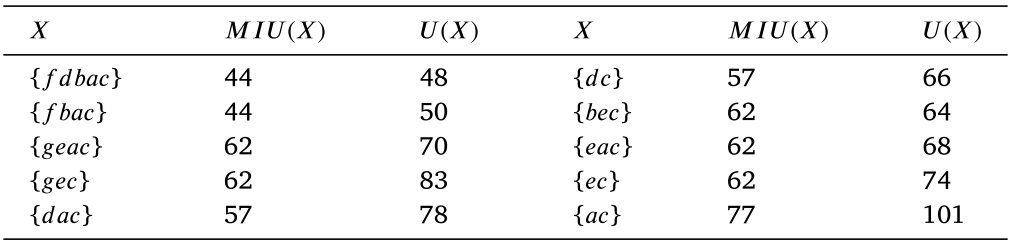
\includegraphics[width=0.9\textwidth]{image/table/table6.PNG}
\caption{\label{fig:table6} Tập HUI kết quả}
\end{figure}

\begin{figure}[h]
\centering
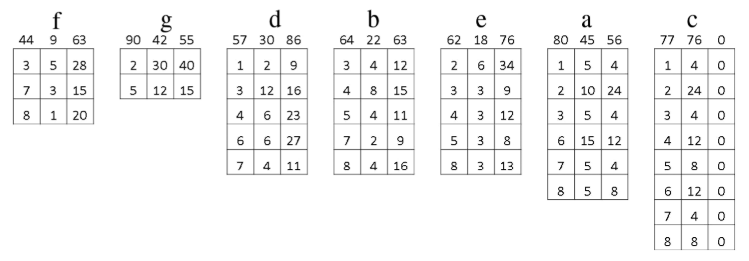
\includegraphics[width=0.95\textwidth]{image/algo/1itemset.PNG}
\caption{\label{fig:1itemset} Bảng 1-itemset}
\end{figure}

\section{Thuật toán MHUI}

\subsection{Mã giả các thuật toán}

\input{chapter/algo.tex}

\subsection{Các phương pháp cắt tỉa cây}

\paragraph{TWU-M-Prune} Nếu $TWU(X) < SMU(X)$ thì những itemset có chứa X (superset của X) không phải là HUI. TWU-M-Prune thực hiện ở dòng 6 trong hình \ref{fig:algo1}.

\paragraph{U-M-Prune} Nếu tổng giá trị tiện ích hậu tố của itemset X nhỏ hơn SMU(X) thì những itemset chứa X (superset của X) không phải HUI. Cụ thể $U(X) + RU(X) < SMU(X)$ thì những itemset chứa X không phải HUI. U-M-Prune thực hiện ở dòng 3 trong hình \ref{fig:algo2}.

\paragraph{EUCS-M-Prune} Nếu EUCS của 2-itemset X nhỏ hơn SMU(X) thì những itemset có chứa X (superset của X) không phải là HUI. 

\paragraph{LA-M-Prune} Phương pháp tỉa cây này sử dụng cả 2 itemset là X và Y, được dùng trong thuật toán xây dựng Utility List (hình \ref{fig:algo3}. Có thể hiểu như sau: 

\begin{itemize}
  \item Tính tổng = $U(X) + RU(X)$ (dòng 2)
  \item Nếu một giao dịch $T_j$ chứa itemset X mà không chứa itemset Y thì giảm tổng đi $U(X, T_j) + RU(X, T_j)$ (điều kiện if dòng 4, phép tính dòng 14) 
  \item Nếu tổng đó nhỏ hơn SMU(X) thì ta cắt bỏ X và kết luận những itemset có chứa X (superset của X) không phải là HUI
\end{itemize}


% % Commands to include a figure:
\begin{figure}[h]
\centering

\includegraphics[width=0.5\textwidth]{image/node.PNG}
\caption{\label{fig:node} Nút}
\end{figure}


% chuong 3
\section{Chèn đoạn code}


ví dụ code \ref{lst:vdcode} là code python 


\begin{lstlisting}[caption={Đoạn code}, label={lst:vdcode}, language=python]
s = "I am Pusheen the cat"
print(s)
\end{lstlisting}

ví dụ trích dẫn \cite{robinson2013graph}


\bibliographystyle{IEEEtran}
\bibliography{bib}

%%%%%%%%%%%%%%%%%%%%%%%%%%%%%%%%%%%%%%%%%%%%%%%%%%%%
% Comments can be added to the margins of the document using the \todo{Here's a comment in the margin!} todo command, as shown in the example on the right. You can also add inline comments too:

% \todo[inline, color=green!40]{This is an inline comment.}



% \subsection{Tables and Figures}

% Use the table and tabular commands for basic tables --- see Table~\ref{tab:widgets}, for example. You can upload a figure (JPEG, PNG or PDF) using the files menu. To include it in your document, use the includegraphics command as in the code for Figure~\ref{fig:frog} below.

% % % Commands to include a figure:
% % \begin{figure}
% % \centering
% % 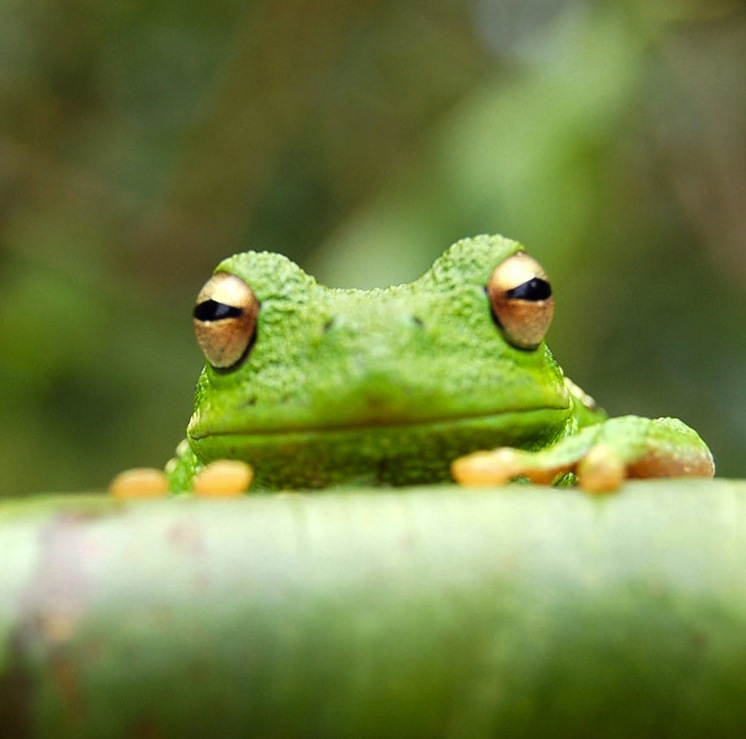
\includegraphics[width=0.5\textwidth]{frog.jpg}
% % \caption{\label{fig:frog}This is a figure caption.}
% % \end{figure}

% % \begin{table}
% % \centering
% % \begin{tabular}{l|r}
% % Item & Quantity \\\hline
% % Widgets & 42 \\
% % Gadgets & 13
% % \end{tabular}
% % \caption{\label{tab:widgets}An example table.}
% % \end{table}

% \subsection{Mathematics}

% \LaTeX{} is great at typesetting mathematics. Let $X_1, X_2, \ldots, X_n$ be a sequence of independent and identically distributed random variables with $\text{E}[X_i] = \mu$ and $\text{Var}[X_i] = \sigma^2 < \infty$, and let
% $$S_n = \frac{X_1 + X_2 + \cdots + X_n}{n}
%       = \frac{1}{n}\sum_{i}^{n} X_i$$
% denote their mean. Then as $n$ approaches infinity, the random variables $\sqrt{n}(S_n - \mu)$ converge in distribution to a normal $\mathcal{N}(0, \sigma^2)$.

% \subsection{Lists}

% You can make lists with automatic numbering \dots

% \begin{enumerate}
% \item Like this,
% \item and like this.
% \end{enumerate}
% \dots or bullet points \dots
% \begin{itemize}
% \item Like this,
% \item and like this.
% \end{itemize}

% We hope you find write\LaTeX\ useful, and please let us know if you have any feedback using the help menu above.

\end{document} to your LaTeX file where you want your
% title page.
%t
%%%%%%%%%%%%%%%%%%%%%%%%%%%%%%%%%%%%%%%%%
\title{Template báo cáo KHTN}
%----------------------------------------------------------------------------------------
%	PACKAGES AND OTHER DOCUMENT CONFIGURATIONS
%----------------------------------------------------------------------------------------

\documentclass[12pt]{article}
\usepackage[T5]{fontenc}
\usepackage[utf8]{inputenc}
\usepackage[vietnamese,english]{babel}
\usepackage{amsmath}
\usepackage{graphicx}
\usepackage[colorinlistoftodos]{todonotes}
\usepackage{listings}
\usepackage{hyperref}
\hypersetup{
    colorlinks=true,
    linkcolor=blue,
    filecolor=magenta,      
    urlcolor=cyan,
}

% change name 
\renewcommand{\lstlistingname}{Mã }% Listing -> Algorithm
\addto\captionsenglish{\renewcommand{\figurename}{Hình}} % figure -> Hình 

\begin{document}

\begin{titlepage}

\newcommand{\HRule}{\rule{\linewidth}{0.5mm}} % Defines a new command for the horizontal lines, change thickness here

\center % Center everything on the page
 
%----------------------------------------------------------------------------------------
%	HEADING SECTIONS
%----------------------------------------------------------------------------------------

\textsc{\LARGE Đại học Khoa học tự nhiên}\\[1.5cm] % Name of your university/college
\textsc{\Large Ngành hệ thống thông tin}\\[0.5cm] % Major heading such as course name
\textsc{\large Môn học: Khám phá tri thức và khai thác dữ liệu }\\[0.5cm] % Minor heading such as course title

%----------------------------------------------------------------------------------------
%	TITLE SECTION
%----------------------------------------------------------------------------------------

\HRule \\[0.4cm]
{ \LARGE \bfseries Báo cáo cuối kỳ}\\[0.4cm]
{ \huge \bfseries Tìm hiểu bài báo}\\[0.2cm] % Title of your document
{ \huge \bfseries Efficient mining of high utility itemsets with multiple minimum utility thresholds}\\[0.4cm] % Title of your document
\HRule \\[1.5cm]
 
%----------------------------------------------------------------------------------------
%	AUTHOR SECTION
%----------------------------------------------------------------------------------------

\begin{minipage}{0.4\textwidth}
\begin{flushleft} \large
\emph{Học viên:}\\
Thái Thiện  -- 17C12031 % Your name
\end{flushleft}
\end{minipage}
~
\begin{minipage}{0.4\textwidth}
\begin{flushright} \large
\emph{Giảng viên:} \\
PGS.TS. LÊ HOÀI BẮC % Supervisor's Name
\end{flushright}
\end{minipage}\\[2cm]

% If you don't want a supervisor, uncomment the two lines below and remove the section above
%\Large \emph{Author:}\\
%John \textsc{Smith}\\[3cm] % Your name

%----------------------------------------------------------------------------------------
%	DATE SECTION
%----------------------------------------------------------------------------------------

% I don't want day because it is English
% {\large \today}\\[2cm] % Date, change the \today to a set date if you want to be precise

%----------------------------------------------------------------------------------------
%	LOGO SECTION
%----------------------------------------------------------------------------------------


\includegraphics{logo/rsz_3logo-khtn.png}\\[1cm] % Include a department/university logo - this will require the graphicx package
 
%----------------------------------------------------------------------------------------

\vfill % Fill the rest of the page with whitespace

\end{titlepage}


\section{Giới thiệu}
Báo cáo này sẽ trình bày về bài báo "Efficient mining of high utility itemsets with multiple minimum utility thresholds" \cite{krishnamoorthy2018efficient} của tác giả Srikumar Krishnamoorthy, thuộc đơn vị Học viện Quản lý Ahmedabad, Ấn Độ. Bài báo đăng trong tập chí Engineering Applications of Artificial Intelligence, năm 2018. 


\section{Các định nghĩa về ký hiệu và bài toán}

\subsection{Định nghĩa}
% from def 1 -> 17

Cho tập $ I = \{i_1, i_2, ..., i_m\}$ là tập các món hàng (item) khác nhau. Một giao dịch (transaction) $T_j = \{x_l | 1, 2, ...N_j, x_l \in I \} $ với $N_j$ là số hàng trong giao dịch  $T_j$. Một cơ sở dữ liệu (database) $D$ có chứa các giao dịch, $D = \{T_1, T_2, ..., T_m\}$, với $m$ số các giao dịch trong cơ sở dữ liệu. Một tập hợp chưa các món hàng $X =\{ x_1, x_2, ... x_k \} \subset I, x_i \in I $ gọi là k-itemset. 

Hình \ref{fig:table2} là một cơ sở dữ liệu D chứa thông tin các giao dịchụ. Hình \ref{fig:table3} là lợi nhuận mỗi đơn vị của mỗi món hàng, và giá trị sử dụng tối thiểu được cho trước.



\begin{figure}[h]
\centering
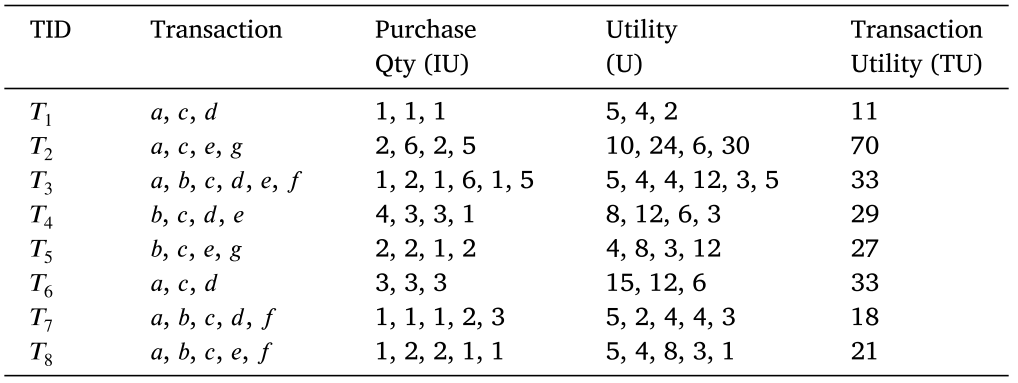
\includegraphics[width=0.9\textwidth]{image/table/table2.PNG}
\caption{\label{fig:table2} Cơ sở dữ liệu}
\end{figure}

\begin{figure}[h]
\centering
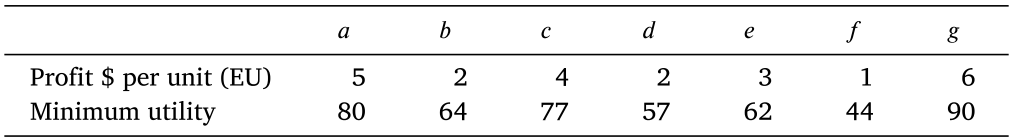
\includegraphics[width=0.9\textwidth]{image/table/table3.PNG}
\caption{\label{fig:table3} Lợi nhuận và giá trị sử dụng tối thiểu}
\end{figure}

\paragraph{Định nghĩa 1}: $ MU(x_i) $ là giá trị tiện ít tối thiểu (minimum utility threshold) của món hàng $x_i$. Thực tế, giá trị tiện ích tối thiểu của món hàng thể hiện hạn mức quan trọng của người dùng đối với món hàng đó. Trong quá trình khai thác, ta tính giá trị tiện ích của mỗi món hàng. Nếu giá trị tiện ích dưới giá trị tiện ích tối thiểu, ta không xét món hàng đó nữa. 

\paragraph{Định nghĩa 2} $MIU(X)$ là giá trị tiện ích tối thiểu của k-itemset, là $MU(x)$ với $x$ là món hàng có giá trị tiện ích tối thiểu nhỏ nhất. $MIU(X) = min \{MU(x_j|x_j \in X\}$ . Ví dụ: $MIU(a) = 80$, $MIU(af) = min\{MU(a), MU(f)\} = 44$


\paragraph{Định nghĩa 3} Chỉ số support của itemset X trong cơ sở dữ liệu D kí hiệu là $Sup(X)$. Support của itemset là tỉ lệ của tần số xuất hiện của itemsetX và tổng số giao dịch n. Ví dụ: $Sup(ac) = 6/8$

\paragraph{Định nghĩa 4} Mỗi món hàng $x_i \in I$ đều có giá trị tiện ích ngoài (external utility value), ký hiệu là $EU(x_i)$. Ví dụ: trong hình \ref{fig:table3} $EU(b) = 2$

\paragraph{Định nghĩa 5} Mỗi món hàng $x_i \in T_j$ có giá trị tiện ích bên trong (internal utility value), kí hiệu là $IU(x_i, T_j)$. Ví dụ: trong hình \ref{fig:table2}, $UI(b, T_3) = 2$

\paragraph{Định nghĩa 6} Giá trị tiện ích của món hàng $x_i \in T_j$ kí hiệu $U(x_i, T_j)$ là tích của giá trị tiện ích ngoài và giá trị tiện ích bên trong. 

$$ U(x_i, T_j) = EU(x_i) \times IU(x_i, T_j) $$ .

Ví dụ: $U(b, T_3) = EU(b) \times IU(b, T_3) = 2 \times 2 = 4$

Giá trị tiện ích thể hiện mức độ quan trọng của món hàng về số lượng được mua (giá trị tiện ích trong) và lợi nhuận mỗi đơn vị (giá trị tiện ích ngoài)

\paragraph{Định nghĩa 7} Giá trị tiện ích của itemset X trong giao dịch $T_j$ là tổng giá trị tiện ích của mỗi món hàng trong itemset đó. 
$$U(X, T_j) = \sum_{x_i \in X} U(x_i, T_j)$$
Ví dụ: trong hình \ref{fig:table2}, $U(ac, T_1) = 5 + 4 = 9$

\paragraph{Định nghĩa 8} $U(X)$ giá trị tiện ích của itemset X trong cơ sở dữ liệu D, bằng tổng giá trị tiện ích của itemset X trong mỗi giao dịch $T_j$

$$ U(X) = \sum_{x_i \subseteq T_j \in D} U(X, T_j) $$

Ví dụ: $U(ac) = U(ac, T_1) + U(ac, T_2) + U(ac, T_3) + U(ac, T_6) + U(ac, T_7) + U(ac, T_8) = 9 + 34 + 9 + 28 + 9 + 13 = 101 $

\paragraph{Định nghĩa 9} Tiện ích của giao dịch $TU(T_j)$ là tổng tiện ích của mỗi món hàng trong giao dịch j.

$$ TU(T_j) = \sum_{X \subseteq T_j and x_i \in X} U(x_i, T_j) $$

Ví dụ: $TU(T_5) = U(b, T_5) + U(c, T_5) + U(e, T_5) + U(g, T_5) = 27$

\paragraph{Định nghĩa 10}  $TWU(X)$ là trọng số giao dịch tiện ích (transaction weighted utility) của itemset X , bằng tổng tiện ích của các giao dịch có chứa itemset X.

$$ TWU(X) = \sum_{X \subseteq T_j \in D} TU(T_j) $$

Giá trị $TWU$ của từng món hàng ghi trong hình \ref{fig:table4}.



\begin{figure}[h]
\centering
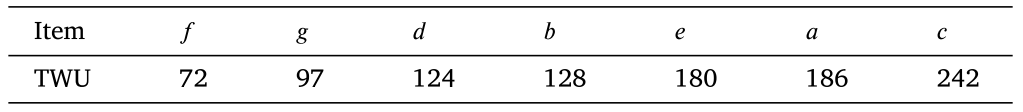
\includegraphics[width=0.9\textwidth]{image/table/table4.PNG}
\caption{\label{fig:table4} Trọng số giao dịch tiện ích  }
\end{figure}

\paragraph{Định nghĩa 11} $T_j/X$ là tập hợp các món hàng sau $X$ trong $T_j$. Ví dụ: trong hình \ref{fig:table2}, $T_i/ac = d, T_7/ac = df$.

\paragraph{Định nghĩa 12} $RU(X, T_j)$  là tiện ích còn lại (remaining utility) của itemset X trong giao dịch $T_j(X \subseteq T_j)$.

$$ RU(X, T_j) = \sum_{x_i \in (T_j/X)} U(x_i, T_j) $$

Ví dụ, trong hình \ref{fig:table2}, $RU(ac, T_1) = 2, RU(ac, T_7) = 4 + 3 = 7 $  

\paragraph{Định nghĩa 13} $RU(X)$ là tiện ích còn lại của itemset X trong cơ sở dữ liệu D, tính bằng tổng các tiện ích còn lại của X ở mỗi giao dịch $T_j$

$$ RU(X) = \sum_{X \subseteq T_j \in D} RU(x, T_j) $$

Ví dụ, trong hình \ref{fig:table2}, $RU(ac) = 2 + 36 + 20 + 6 + 7 + 4 = 75$

\paragraph{Định nghĩa 14} (Về thứ tự các món hàng). Các món hàng trong cơ sở dữ liệu các giao dịch được xử lý theo thứ tự $\succ$ xếp theo giá trị TWU tăng dần. Trong ví dụ của bài báo thứ tự là $ f \succ g \succ d \succ b \succ e \succ a \succ c $. Hình \ref{fig:table5} là cơ sở dữ liệu với mỗi giao dịch đã được sắp xếp các món hàng theo thứ tự TWU. 

\begin{figure}[h]
\centering
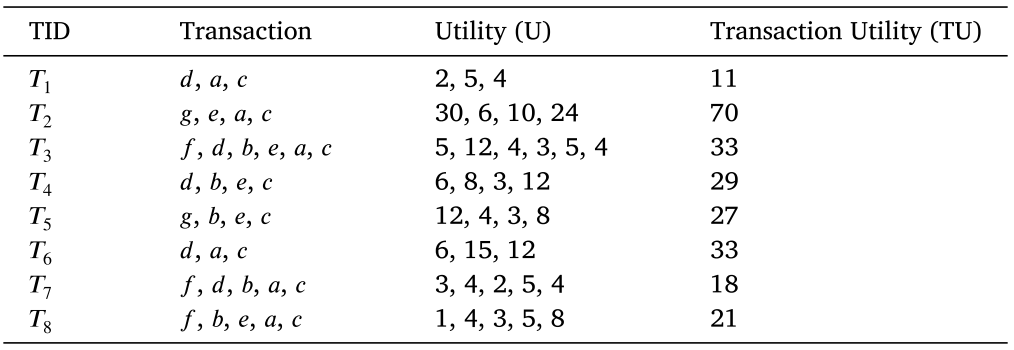
\includegraphics[width=0.9\textwidth]{image/table/table5.PNG}
\caption{\label{fig:table5} Cơ sở dữ liệu sau khi sắp xếp theo TWU  }
\end{figure}

\paragraph{Định nghĩa 15} (Về phần mở rộng của itemset). $Ext(X)$ là phần mở rộng của itemset X, là tất cả các món hàng sau X trong tập hợp các món hàng được xếp theo thứ tự. Ví dụ: $Ext(b) = \{ e, a, c \}$ và $Ext(fd) = \{b, e, a, c \}$.

\paragraph{Định nghĩa 16} $SMU(X)$ là hậu tố tiện ích tối thiểu (suffix minimum utility) của X. 

$$ SMU(U) = min(MIU(X), MIU(Ext(X))) $$

Ví dụ, $SMU(ea) = min(MIU(ea), MIU(Ext(ea))) = min (MIU(ea), MIU(c)) = min(min(62, 80), 77) = 62$

\paragraph{Định nghĩa 17} EUCS, cấu trúc đồng xảy ra tiện ích ước tính (Estimated Utility Co-occurrence Structure) \cite{fournier2014fhm} là một ma trận tam giác như hình \ref{fig:eucs}. Ma trận này để chứa giá trị TWU của một cặp itemset. 

\begin{figure}[h]
\centering
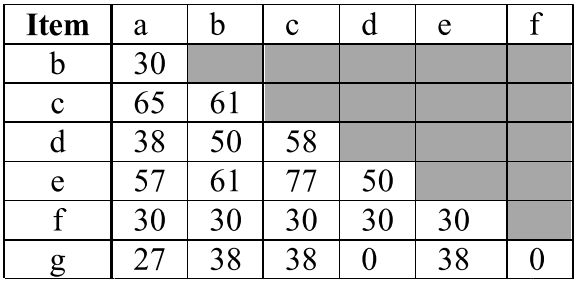
\includegraphics[width=0.7\textwidth]{image/fig/trianglematrix.PNG}
\caption{\label{fig:eucs} Ma trận tam giác  }
\end{figure} 

\subsection{Định nghĩa bài toán}

\paragraph{Dữ liệu đầu vào} Cơ sở dữ liệu D chứa các giao dịch, $D = \{T_1, T_2, ..., T_m\}$, giá trị tiện ích trong và ngoài của mỗi món hàng, và ngưỡng giá trị tiện ích tối thiểu. (như trong hình \ref{fig:table2} và hình \ref{fig:table3}).

\paragraph{Dữ liệu đầu ra} Tập HUI (high utility itemset) bao gồm các itemset X có giá trị tiện ích cao hơn giá trị tiện ích tối thiểu của itemset đó (như hình \ref{fig:table6}). HUI định nghĩa như sau

$$HUI = \{ X : U(X) | X \subseteq I, U(X) \geq MIU(X) \} $$

\begin{figure}[h]
\centering
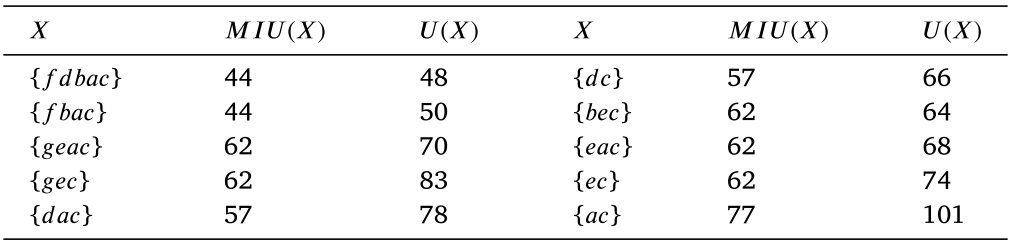
\includegraphics[width=0.9\textwidth]{image/table/table6.PNG}
\caption{\label{fig:table6} Tập HUI kết quả}
\end{figure}

\begin{figure}[h]
\centering
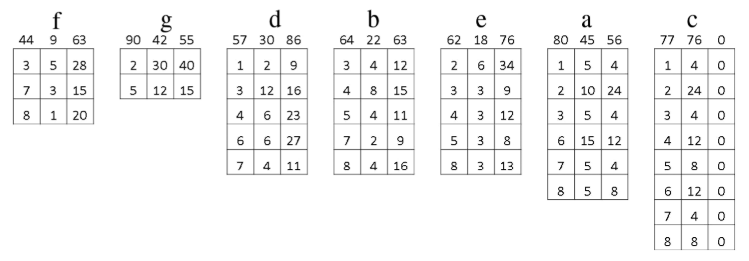
\includegraphics[width=0.95\textwidth]{image/algo/1itemset.PNG}
\caption{\label{fig:1itemset} Bảng 1-itemset}
\end{figure}

\section{Thuật toán MHUI}

\subsection{Mã giả các thuật toán}


\subsubsection{MHUI main}

\begin{figure}[ht]
\centering
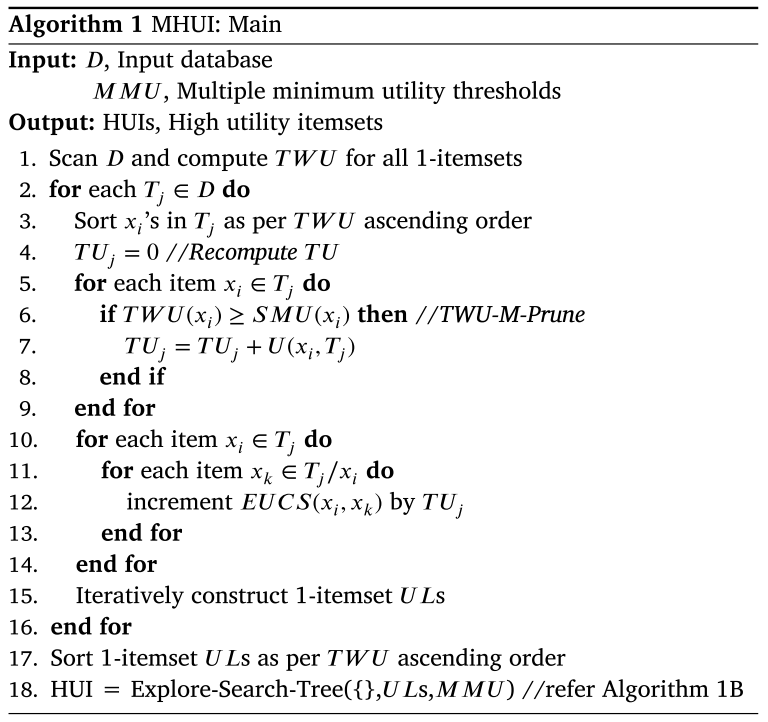
\includegraphics[width=0.9\textwidth]{image/algo/algo1.PNG}
\caption{\label{fig:algo1} MHUI main}
\end{figure}

\paragraph{Dữ liệu đầu vào} Cơ sở dữ liệu D, ngưỡng giá trị hữu dụng tối thiểu cho từng món hàng.  
\paragraph{Dữ liệu đầu ra} HUIs, tập các itemset có giá trị hữu dụng cao.\\



Hình \ref{fig:algo1} là hàm bắt đầu chương trình. Chương trình sẽ tính các TWU (tạo ra bảng như hình\ref{fig:table4}), dòng 1 trong thuật toán, đây là lần duyệt cơ sở dữ liệu đầu tiên. Sau đó, chương trình duyệt qua cơ sở dữ liệu lần 2, ở mỗi giao dịch $T_j$ chương trình sẽ làm những việc sau đây trong mỗi vòng lập qua 1 giao dịch.

\begin{itemize}
  \item Sắp xếp các món hàng trong giao dịch theo thứ tự TWU (dòng 3). 
  \item Tính lại TU cho mỗi giao dịch sau khi áp dụng phương pháp tỉa cây TWU-M-Prune. (dòng 6, 7)
  \item Tính EUCS dựa vào TU sau khi tỉa cây TWU-M-Prune (dòng 12)
  \item Từ từ xây dựng 1-itemset utility list (gọi tắt ULs) như hình \ref{fig:1itemset} (dòng 15) 
\end{itemize}

Sau khi kết thức vòng lập, sắp xếp ULs theo thứ tự TWU (dòng 17), gọi hàm Explore-Search-Tree (dòng 18). 

\subsubsection{Hàm duyệt cây: Explore-Search-Tree }

\begin{figure}[ht]
\centering
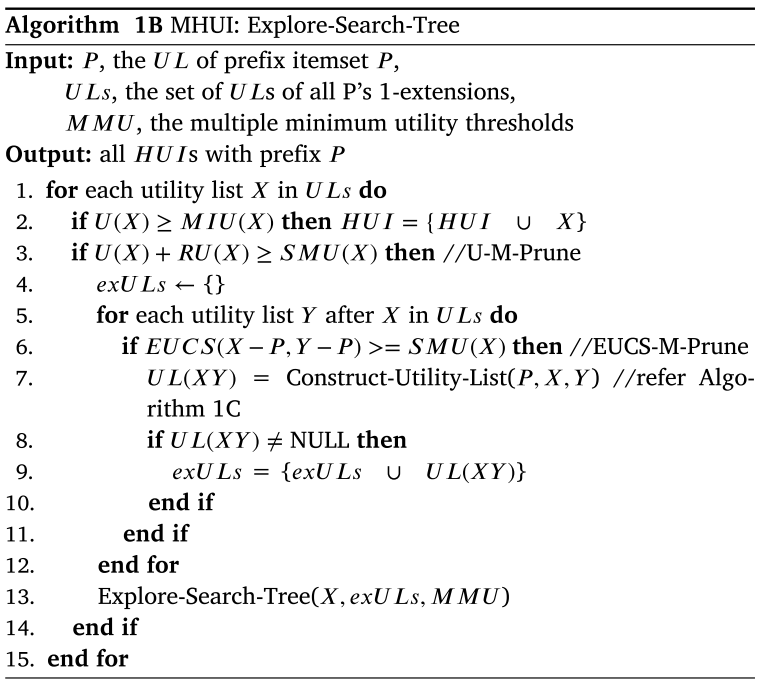
\includegraphics[width=0.9\textwidth]{image/algo/algo2.PNG}
\caption{\label{fig:algo2} MHUI Explore Search Tree}
\end{figure}

\paragraph{Dữ liệu đầu vào} Một itemset gọi là P, tập hợp có thứ tự các itemset ULs, ngưỡng giá trị hữu dụng tối thiểu cho từng món hàng.

\paragraph{Dữ liệu đầu ra} HUIs với tiền tố P \\

Hàm duyệt cây (hình \ref{fig:algo2}) sẽ kiểm tra cái nút tại đó xem nó có là HUI không (có $U(X) \geq MIU(X)$ ) đê gắn nút vào danh sách HUI trả về cuối cùng. Hàm duyệt cây theo Depth First Search, nghĩa là nó sẽ duyệt một nút sâu nhất có thể, sau đó mới chuyển qua nút tiếp theo. Một nút chỉ được duyệt khi nó thỏa U-M-Prune. 

Quá trình duyệt cây sẽ lập qua mỗi X trong tập ULs. Nếu X thóa U-M-Prune, rồi vòng lập con lập qua mỗi Y theo sau X trong ULs (ULs đã xếp theo thứ tự TWU), và thực hiện 2 việc sau 

\begin{itemize}
  \item kiểm tra P, X, Y thỏa EUCS-M-Prune (dòng 6), bỏ qua vòng lập này nếu không thỏa   
  \item xây dựng danh sách UL (dòng 7). Sẽ gọi hàm \ref{fig:algo3} để tạo ra UL. 
  \item gộp vào dãy exULs (dòng 8) 
\end{itemize}
 
Sau mỗi vòng lập ngoài (vòng lập của X) thuật toán gọi đệ quy gọi đệ quy Explore-Search-Tree(X, exULs) để duyệt cây theo depth first search. 

\subsubsection{Xây dựng dãy hữu dụng: Construct-Utility-List }

\paragraph{Dữ liệu đầu vào} UL itemset P, itemset Px, và itemset Py 

\paragraph{Dữ liệu đầu ra} UL của itemset Pxy \\

\begin{figure}[ht]
\centering
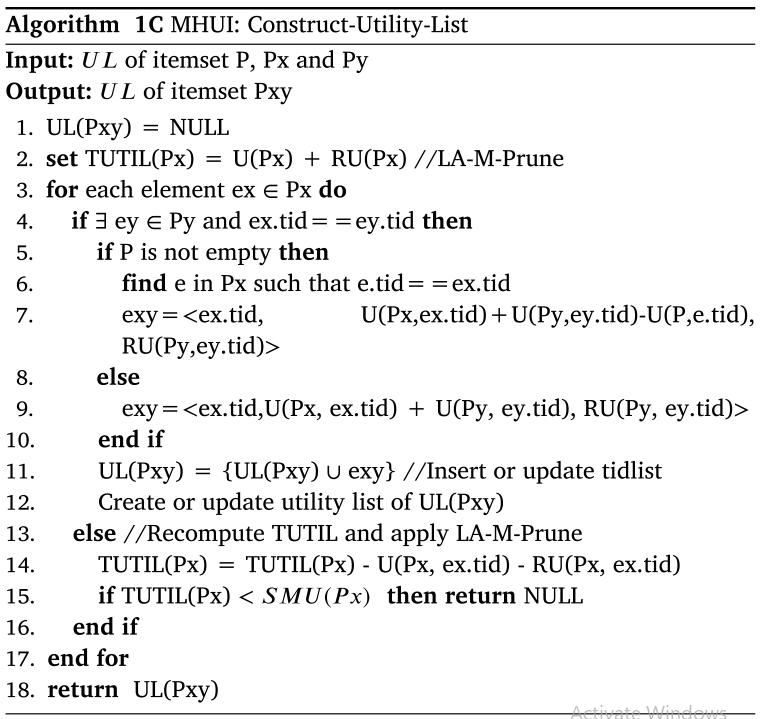
\includegraphics[width=0.9\textwidth]{image/algo/algo3.PNG}
\caption{\label{fig:algo3} MHUI Construct Utility List}
\end{figure}

Thuật toán tạo dãy Utility như hình \ref{fig:algo3} sẽ tạo ra UL mới từ 2 bằng cách ghép 2 UL Px và Py. Cả 2 UL Px và Py đều có chung tiền tố P. Thuật toán sẽ áp dụng LA-M-Prune và trả về NULL (rỗng) khi Px và Py không thỏa điều kiện. 

Kết quả trả về sẽ như một cột như hình \ref{fig:1itemset}, bao gồm itemset và mỗi dãy các bảng ghi có dạng <tid, U, RU>. 


\subsection{Các phương pháp cắt tỉa cây}

\paragraph{TWU-M-Prune} Nếu $TWU(X) < SMU(X)$ thì những itemset có chứa X (superset của X) không phải là HUI. TWU-M-Prune thực hiện ở dòng 6 trong hình \ref{fig:algo1}.

\paragraph{U-M-Prune} Nếu tổng giá trị tiện ích hậu tố của itemset X nhỏ hơn SMU(X) thì những itemset chứa X (superset của X) không phải HUI. Cụ thể $U(X) + RU(X) < SMU(X)$ thì những itemset chứa X không phải HUI. U-M-Prune thực hiện ở dòng 3 trong hình \ref{fig:algo2}.

\paragraph{EUCS-M-Prune} Nếu EUCS của 2-itemset X nhỏ hơn SMU(X) thì những itemset có chứa X (superset của X) không phải là HUI. 

\paragraph{LA-M-Prune} Phương pháp tỉa cây này sử dụng cả 2 itemset là X và Y, được dùng trong thuật toán xây dựng Utility List (hình \ref{fig:algo3}. Có thể hiểu như sau: 

\begin{itemize}
  \item Tính tổng = $U(X) + RU(X)$ (dòng 2)
  \item Nếu một giao dịch $T_j$ chứa itemset X mà không chứa itemset Y thì giảm tổng đi $U(X, T_j) + RU(X, T_j)$ (điều kiện if dòng 4, phép tính dòng 14) 
  \item Nếu tổng đó nhỏ hơn SMU(X) thì ta cắt bỏ X và kết luận những itemset có chứa X (superset của X) không phải là HUI
\end{itemize}


% % Commands to include a figure:
\begin{figure}[h]
\centering

\includegraphics[width=0.5\textwidth]{image/node.PNG}
\caption{\label{fig:node} Nút}
\end{figure}


% chuong 3
\section{Chèn đoạn code}


ví dụ code \ref{lst:vdcode} là code python 


\begin{lstlisting}[caption={Đoạn code}, label={lst:vdcode}, language=python]
s = "I am Pusheen the cat"
print(s)
\end{lstlisting}

ví dụ trích dẫn \cite{robinson2013graph}


\bibliographystyle{IEEEtran}
\bibliography{bib}

%%%%%%%%%%%%%%%%%%%%%%%%%%%%%%%%%%%%%%%%%%%%%%%%%%%%
% Comments can be added to the margins of the document using the \todo{Here's a comment in the margin!} todo command, as shown in the example on the right. You can also add inline comments too:

% \todo[inline, color=green!40]{This is an inline comment.}



% \subsection{Tables and Figures}

% Use the table and tabular commands for basic tables --- see Table~\ref{tab:widgets}, for example. You can upload a figure (JPEG, PNG or PDF) using the files menu. To include it in your document, use the includegraphics command as in the code for Figure~\ref{fig:frog} below.

% % % Commands to include a figure:
% % \begin{figure}
% % \centering
% % 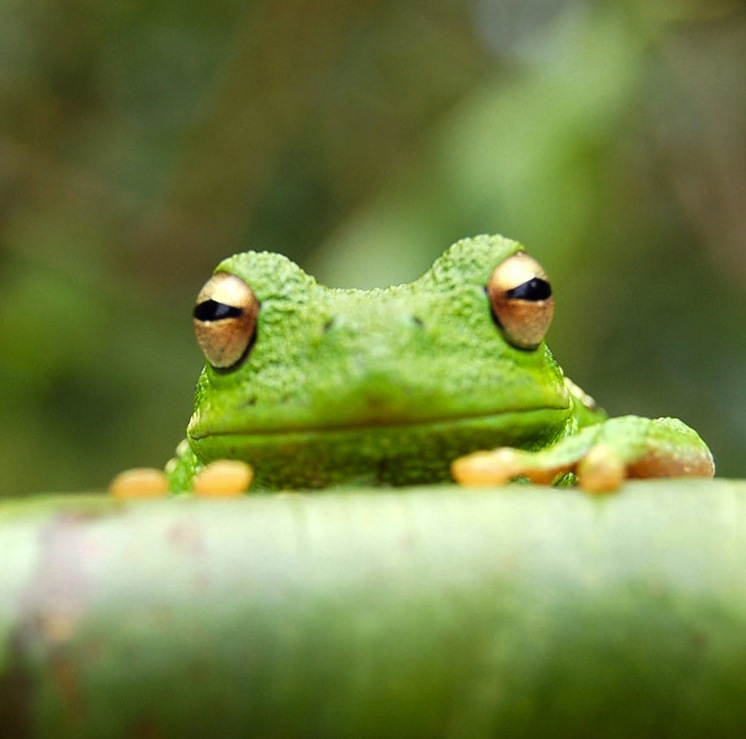
\includegraphics[width=0.5\textwidth]{frog.jpg}
% % \caption{\label{fig:frog}This is a figure caption.}
% % \end{figure}

% % \begin{table}
% % \centering
% % \begin{tabular}{l|r}
% % Item & Quantity \\\hline
% % Widgets & 42 \\
% % Gadgets & 13
% % \end{tabular}
% % \caption{\label{tab:widgets}An example table.}
% % \end{table}

% \subsection{Mathematics}

% \LaTeX{} is great at typesetting mathematics. Let $X_1, X_2, \ldots, X_n$ be a sequence of independent and identically distributed random variables with $\text{E}[X_i] = \mu$ and $\text{Var}[X_i] = \sigma^2 < \infty$, and let
% $$S_n = \frac{X_1 + X_2 + \cdots + X_n}{n}
%       = \frac{1}{n}\sum_{i}^{n} X_i$$
% denote their mean. Then as $n$ approaches infinity, the random variables $\sqrt{n}(S_n - \mu)$ converge in distribution to a normal $\mathcal{N}(0, \sigma^2)$.

% \subsection{Lists}

% You can make lists with automatic numbering \dots

% \begin{enumerate}
% \item Like this,
% \item and like this.
% \end{enumerate}
% \dots or bullet points \dots
% \begin{itemize}
% \item Like this,
% \item and like this.
% \end{itemize}

% We hope you find write\LaTeX\ useful, and please let us know if you have any feedback using the help menu above.

\end{document} to your LaTeX file where you want your
% title page.
%t
%%%%%%%%%%%%%%%%%%%%%%%%%%%%%%%%%%%%%%%%%
\title{Template báo cáo KHTN}
%----------------------------------------------------------------------------------------
%	PACKAGES AND OTHER DOCUMENT CONFIGURATIONS
%----------------------------------------------------------------------------------------

\documentclass[12pt]{article}
\usepackage[T5]{fontenc}
\usepackage[utf8]{inputenc}
\usepackage[vietnamese,english]{babel}
\usepackage{amsmath}
\usepackage{graphicx}
\usepackage[colorinlistoftodos]{todonotes}
\usepackage{listings}
\usepackage{hyperref}
\hypersetup{
    colorlinks=true,
    linkcolor=blue,
    filecolor=magenta,      
    urlcolor=cyan,
}

% change name 
\renewcommand{\lstlistingname}{Mã }% Listing -> Algorithm
\addto\captionsenglish{\renewcommand{\figurename}{Hình}} % figure -> Hình 

\begin{document}

\begin{titlepage}

\newcommand{\HRule}{\rule{\linewidth}{0.5mm}} % Defines a new command for the horizontal lines, change thickness here

\center % Center everything on the page
 
%----------------------------------------------------------------------------------------
%	HEADING SECTIONS
%----------------------------------------------------------------------------------------

\textsc{\LARGE Đại học Khoa học tự nhiên}\\[1.5cm] % Name of your university/college
\textsc{\Large Ngành hệ thống thông tin}\\[0.5cm] % Major heading such as course name
\textsc{\large Môn học: Khám phá tri thức và khai thác dữ liệu }\\[0.5cm] % Minor heading such as course title

%----------------------------------------------------------------------------------------
%	TITLE SECTION
%----------------------------------------------------------------------------------------

\HRule \\[0.4cm]
{ \LARGE \bfseries Báo cáo cuối kỳ}\\[0.4cm]
{ \huge \bfseries Tìm hiểu bài báo}\\[0.2cm] % Title of your document
{ \huge \bfseries Efficient mining of high utility itemsets with multiple minimum utility thresholds}\\[0.4cm] % Title of your document
\HRule \\[1.5cm]
 
%----------------------------------------------------------------------------------------
%	AUTHOR SECTION
%----------------------------------------------------------------------------------------

\begin{minipage}{0.4\textwidth}
\begin{flushleft} \large
\emph{Học viên:}\\
Thái Thiện  -- 17C12031 % Your name
\end{flushleft}
\end{minipage}
~
\begin{minipage}{0.4\textwidth}
\begin{flushright} \large
\emph{Giảng viên:} \\
PGS.TS. LÊ HOÀI BẮC % Supervisor's Name
\end{flushright}
\end{minipage}\\[2cm]

% If you don't want a supervisor, uncomment the two lines below and remove the section above
%\Large \emph{Author:}\\
%John \textsc{Smith}\\[3cm] % Your name

%----------------------------------------------------------------------------------------
%	DATE SECTION
%----------------------------------------------------------------------------------------

% I don't want day because it is English
% {\large \today}\\[2cm] % Date, change the \today to a set date if you want to be precise

%----------------------------------------------------------------------------------------
%	LOGO SECTION
%----------------------------------------------------------------------------------------


\includegraphics{logo/rsz_3logo-khtn.png}\\[1cm] % Include a department/university logo - this will require the graphicx package
 
%----------------------------------------------------------------------------------------

\vfill % Fill the rest of the page with whitespace

\end{titlepage}


\section{Giới thiệu}
Báo cáo này sẽ trình bày về bài báo "Efficient mining of high utility itemsets with multiple minimum utility thresholds" \cite{krishnamoorthy2018efficient} của tác giả Srikumar Krishnamoorthy, thuộc đơn vị Học viện Quản lý Ahmedabad, Ấn Độ. Bài báo đăng trong tập chí Engineering Applications of Artificial Intelligence, năm 2018. 


\section{Các định nghĩa về ký hiệu và bài toán}

\subsection{Định nghĩa}
% from def 1 -> 17

Cho tập $ I = \{i_1, i_2, ..., i_m\}$ là tập các món hàng (item) khác nhau. Một giao dịch (transaction) $T_j = \{x_l | 1, 2, ...N_j, x_l \in I \} $ với $N_j$ là số hàng trong giao dịch  $T_j$. Một cơ sở dữ liệu (database) $D$ có chứa các giao dịch, $D = \{T_1, T_2, ..., T_m\}$, với $m$ số các giao dịch trong cơ sở dữ liệu. Một tập hợp chưa các món hàng $X =\{ x_1, x_2, ... x_k \} \subset I, x_i \in I $ gọi là k-itemset. 

Hình \ref{fig:table2} là một cơ sở dữ liệu D chứa thông tin các giao dịchụ. Hình \ref{fig:table3} là lợi nhuận mỗi đơn vị của mỗi món hàng, và giá trị sử dụng tối thiểu được cho trước.



\begin{figure}[h]
\centering
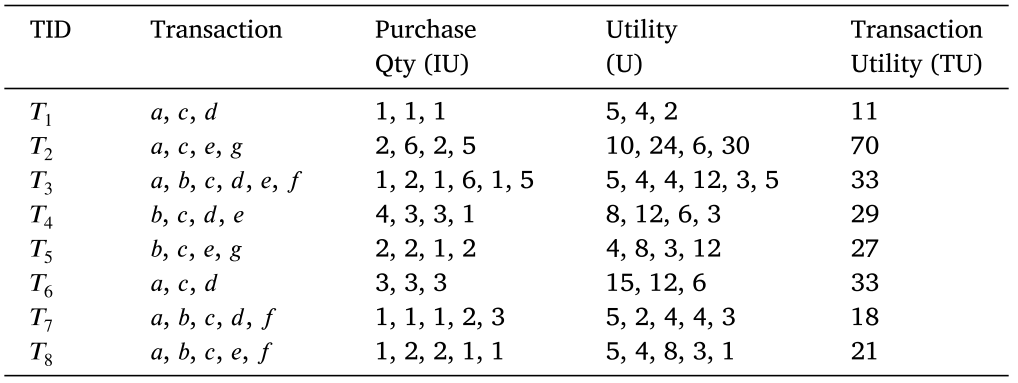
\includegraphics[width=0.9\textwidth]{image/table/table2.PNG}
\caption{\label{fig:table2} Cơ sở dữ liệu}
\end{figure}

\begin{figure}[h]
\centering
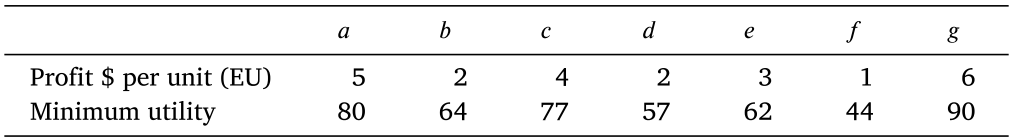
\includegraphics[width=0.9\textwidth]{image/table/table3.PNG}
\caption{\label{fig:table3} Lợi nhuận và giá trị sử dụng tối thiểu}
\end{figure}

\paragraph{Định nghĩa 1}: $ MU(x_i) $ là giá trị tiện ít tối thiểu (minimum utility threshold) của món hàng $x_i$. Thực tế, giá trị tiện ích tối thiểu của món hàng thể hiện hạn mức quan trọng của người dùng đối với món hàng đó. Trong quá trình khai thác, ta tính giá trị tiện ích của mỗi món hàng. Nếu giá trị tiện ích dưới giá trị tiện ích tối thiểu, ta không xét món hàng đó nữa. 

\paragraph{Định nghĩa 2} $MIU(X)$ là giá trị tiện ích tối thiểu của k-itemset, là $MU(x)$ với $x$ là món hàng có giá trị tiện ích tối thiểu nhỏ nhất. $MIU(X) = min \{MU(x_j|x_j \in X\}$ . Ví dụ: $MIU(a) = 80$, $MIU(af) = min\{MU(a), MU(f)\} = 44$


\paragraph{Định nghĩa 3} Chỉ số support của itemset X trong cơ sở dữ liệu D kí hiệu là $Sup(X)$. Support của itemset là tỉ lệ của tần số xuất hiện của itemsetX và tổng số giao dịch n. Ví dụ: $Sup(ac) = 6/8$

\paragraph{Định nghĩa 4} Mỗi món hàng $x_i \in I$ đều có giá trị tiện ích ngoài (external utility value), ký hiệu là $EU(x_i)$. Ví dụ: trong hình \ref{fig:table3} $EU(b) = 2$

\paragraph{Định nghĩa 5} Mỗi món hàng $x_i \in T_j$ có giá trị tiện ích bên trong (internal utility value), kí hiệu là $IU(x_i, T_j)$. Ví dụ: trong hình \ref{fig:table2}, $UI(b, T_3) = 2$

\paragraph{Định nghĩa 6} Giá trị tiện ích của món hàng $x_i \in T_j$ kí hiệu $U(x_i, T_j)$ là tích của giá trị tiện ích ngoài và giá trị tiện ích bên trong. 

$$ U(x_i, T_j) = EU(x_i) \times IU(x_i, T_j) $$ .

Ví dụ: $U(b, T_3) = EU(b) \times IU(b, T_3) = 2 \times 2 = 4$

Giá trị tiện ích thể hiện mức độ quan trọng của món hàng về số lượng được mua (giá trị tiện ích trong) và lợi nhuận mỗi đơn vị (giá trị tiện ích ngoài)

\paragraph{Định nghĩa 7} Giá trị tiện ích của itemset X trong giao dịch $T_j$ là tổng giá trị tiện ích của mỗi món hàng trong itemset đó. 
$$U(X, T_j) = \sum_{x_i \in X} U(x_i, T_j)$$
Ví dụ: trong hình \ref{fig:table2}, $U(ac, T_1) = 5 + 4 = 9$

\paragraph{Định nghĩa 8} $U(X)$ giá trị tiện ích của itemset X trong cơ sở dữ liệu D, bằng tổng giá trị tiện ích của itemset X trong mỗi giao dịch $T_j$

$$ U(X) = \sum_{x_i \subseteq T_j \in D} U(X, T_j) $$

Ví dụ: $U(ac) = U(ac, T_1) + U(ac, T_2) + U(ac, T_3) + U(ac, T_6) + U(ac, T_7) + U(ac, T_8) = 9 + 34 + 9 + 28 + 9 + 13 = 101 $

\paragraph{Định nghĩa 9} Tiện ích của giao dịch $TU(T_j)$ là tổng tiện ích của mỗi món hàng trong giao dịch j.

$$ TU(T_j) = \sum_{X \subseteq T_j and x_i \in X} U(x_i, T_j) $$

Ví dụ: $TU(T_5) = U(b, T_5) + U(c, T_5) + U(e, T_5) + U(g, T_5) = 27$

\paragraph{Định nghĩa 10}  $TWU(X)$ là trọng số giao dịch tiện ích (transaction weighted utility) của itemset X , bằng tổng tiện ích của các giao dịch có chứa itemset X.

$$ TWU(X) = \sum_{X \subseteq T_j \in D} TU(T_j) $$

Giá trị $TWU$ của từng món hàng ghi trong hình \ref{fig:table4}.



\begin{figure}[h]
\centering
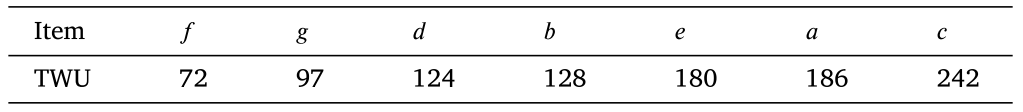
\includegraphics[width=0.9\textwidth]{image/table/table4.PNG}
\caption{\label{fig:table4} Trọng số giao dịch tiện ích  }
\end{figure}

\paragraph{Định nghĩa 11} $T_j/X$ là tập hợp các món hàng sau $X$ trong $T_j$. Ví dụ: trong hình \ref{fig:table2}, $T_i/ac = d, T_7/ac = df$.

\paragraph{Định nghĩa 12} $RU(X, T_j)$  là tiện ích còn lại (remaining utility) của itemset X trong giao dịch $T_j(X \subseteq T_j)$.

$$ RU(X, T_j) = \sum_{x_i \in (T_j/X)} U(x_i, T_j) $$

Ví dụ, trong hình \ref{fig:table2}, $RU(ac, T_1) = 2, RU(ac, T_7) = 4 + 3 = 7 $  

\paragraph{Định nghĩa 13} $RU(X)$ là tiện ích còn lại của itemset X trong cơ sở dữ liệu D, tính bằng tổng các tiện ích còn lại của X ở mỗi giao dịch $T_j$

$$ RU(X) = \sum_{X \subseteq T_j \in D} RU(x, T_j) $$

Ví dụ, trong hình \ref{fig:table2}, $RU(ac) = 2 + 36 + 20 + 6 + 7 + 4 = 75$

\paragraph{Định nghĩa 14} (Về thứ tự các món hàng). Các món hàng trong cơ sở dữ liệu các giao dịch được xử lý theo thứ tự $\succ$ xếp theo giá trị TWU tăng dần. Trong ví dụ của bài báo thứ tự là $ f \succ g \succ d \succ b \succ e \succ a \succ c $. Hình \ref{fig:table5} là cơ sở dữ liệu với mỗi giao dịch đã được sắp xếp các món hàng theo thứ tự TWU. 

\begin{figure}[h]
\centering
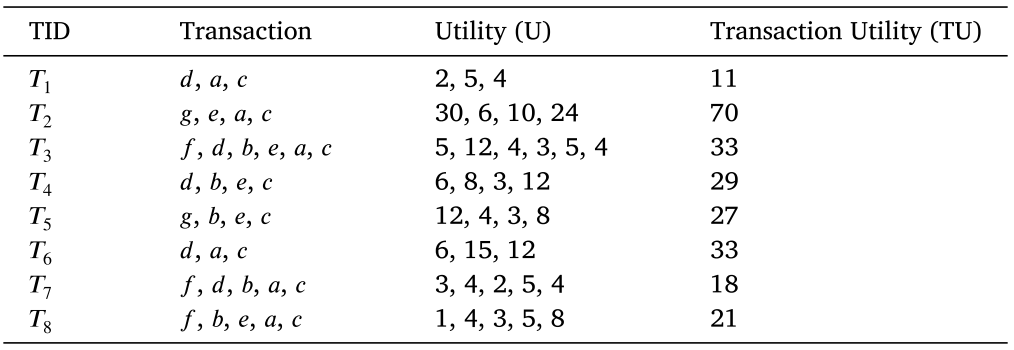
\includegraphics[width=0.9\textwidth]{image/table/table5.PNG}
\caption{\label{fig:table5} Cơ sở dữ liệu sau khi sắp xếp theo TWU  }
\end{figure}

\paragraph{Định nghĩa 15} (Về phần mở rộng của itemset). $Ext(X)$ là phần mở rộng của itemset X, là tất cả các món hàng sau X trong tập hợp các món hàng được xếp theo thứ tự. Ví dụ: $Ext(b) = \{ e, a, c \}$ và $Ext(fd) = \{b, e, a, c \}$.

\paragraph{Định nghĩa 16} $SMU(X)$ là hậu tố tiện ích tối thiểu (suffix minimum utility) của X. 

$$ SMU(U) = min(MIU(X), MIU(Ext(X))) $$

Ví dụ, $SMU(ea) = min(MIU(ea), MIU(Ext(ea))) = min (MIU(ea), MIU(c)) = min(min(62, 80), 77) = 62$

\paragraph{Định nghĩa 17} EUCS, cấu trúc đồng xảy ra tiện ích ước tính (Estimated Utility Co-occurrence Structure) \cite{fournier2014fhm} là một ma trận tam giác như hình \ref{fig:eucs}. Ma trận này để chứa giá trị TWU của một cặp itemset. 

\begin{figure}[h]
\centering
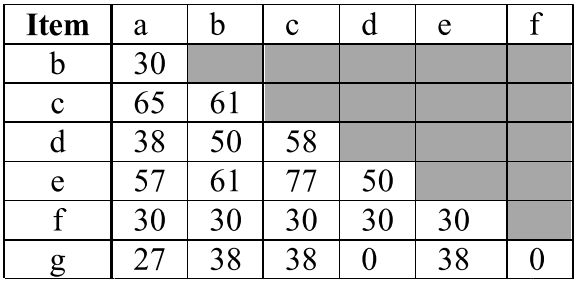
\includegraphics[width=0.7\textwidth]{image/fig/trianglematrix.PNG}
\caption{\label{fig:eucs} Ma trận tam giác  }
\end{figure} 

\subsection{Định nghĩa bài toán}

\paragraph{Dữ liệu đầu vào} Cơ sở dữ liệu D chứa các giao dịch, $D = \{T_1, T_2, ..., T_m\}$, giá trị tiện ích trong và ngoài của mỗi món hàng, và ngưỡng giá trị tiện ích tối thiểu. (như trong hình \ref{fig:table2} và hình \ref{fig:table3}).

\paragraph{Dữ liệu đầu ra} Tập HUI (high utility itemset) bao gồm các itemset X có giá trị tiện ích cao hơn giá trị tiện ích tối thiểu của itemset đó (như hình \ref{fig:table6}). HUI định nghĩa như sau

$$HUI = \{ X : U(X) | X \subseteq I, U(X) \geq MIU(X) \} $$

\begin{figure}[h]
\centering
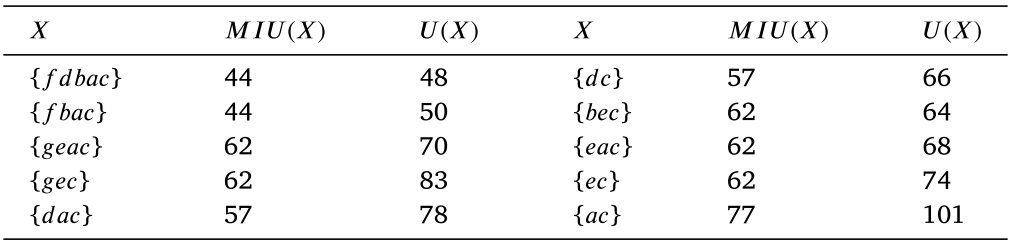
\includegraphics[width=0.9\textwidth]{image/table/table6.PNG}
\caption{\label{fig:table6} Tập HUI kết quả}
\end{figure}

\begin{figure}[h]
\centering
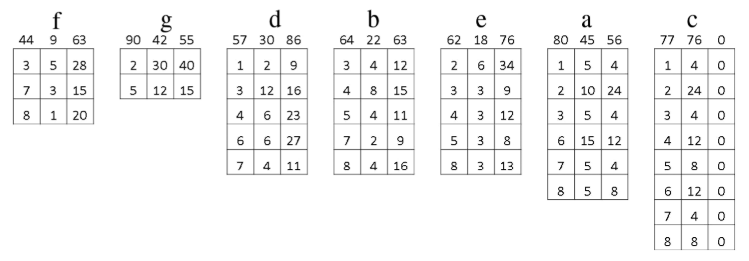
\includegraphics[width=0.95\textwidth]{image/algo/1itemset.PNG}
\caption{\label{fig:1itemset} Bảng 1-itemset}
\end{figure}

\section{Thuật toán MHUI}

\subsection{Mã giả các thuật toán}


\subsubsection{MHUI main}

\begin{figure}[ht]
\centering
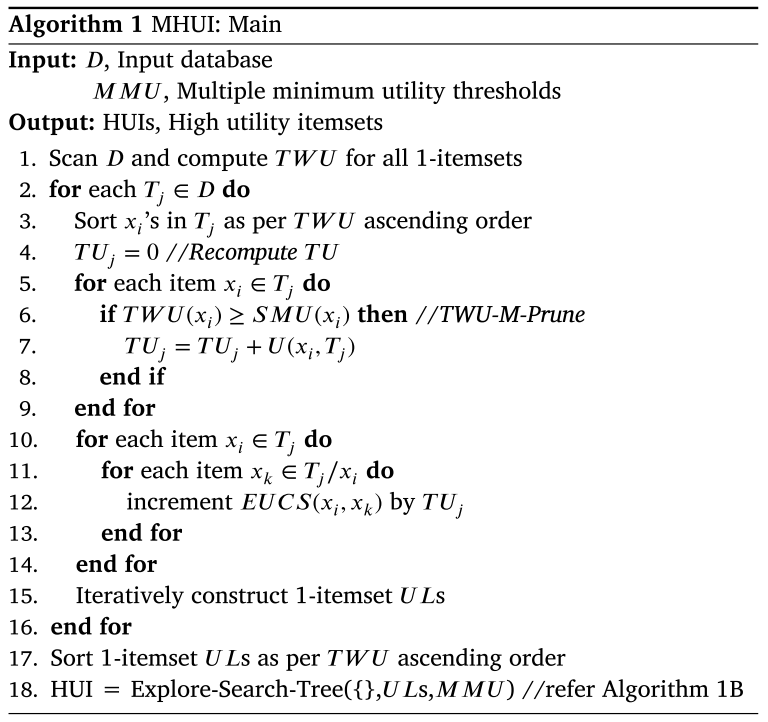
\includegraphics[width=0.9\textwidth]{image/algo/algo1.PNG}
\caption{\label{fig:algo1} MHUI main}
\end{figure}

\paragraph{Dữ liệu đầu vào} Cơ sở dữ liệu D, ngưỡng giá trị hữu dụng tối thiểu cho từng món hàng.  
\paragraph{Dữ liệu đầu ra} HUIs, tập các itemset có giá trị hữu dụng cao.\\



Hình \ref{fig:algo1} là hàm bắt đầu chương trình. Chương trình sẽ tính các TWU (tạo ra bảng như hình\ref{fig:table4}), dòng 1 trong thuật toán, đây là lần duyệt cơ sở dữ liệu đầu tiên. Sau đó, chương trình duyệt qua cơ sở dữ liệu lần 2, ở mỗi giao dịch $T_j$ chương trình sẽ làm những việc sau đây trong mỗi vòng lập qua 1 giao dịch.

\begin{itemize}
  \item Sắp xếp các món hàng trong giao dịch theo thứ tự TWU (dòng 3). 
  \item Tính lại TU cho mỗi giao dịch sau khi áp dụng phương pháp tỉa cây TWU-M-Prune. (dòng 6, 7)
  \item Tính EUCS dựa vào TU sau khi tỉa cây TWU-M-Prune (dòng 12)
  \item Từ từ xây dựng 1-itemset utility list (gọi tắt ULs) như hình \ref{fig:1itemset} (dòng 15) 
\end{itemize}

Sau khi kết thức vòng lập, sắp xếp ULs theo thứ tự TWU (dòng 17), gọi hàm Explore-Search-Tree (dòng 18). 

\subsubsection{Hàm duyệt cây: Explore-Search-Tree }

\begin{figure}[ht]
\centering
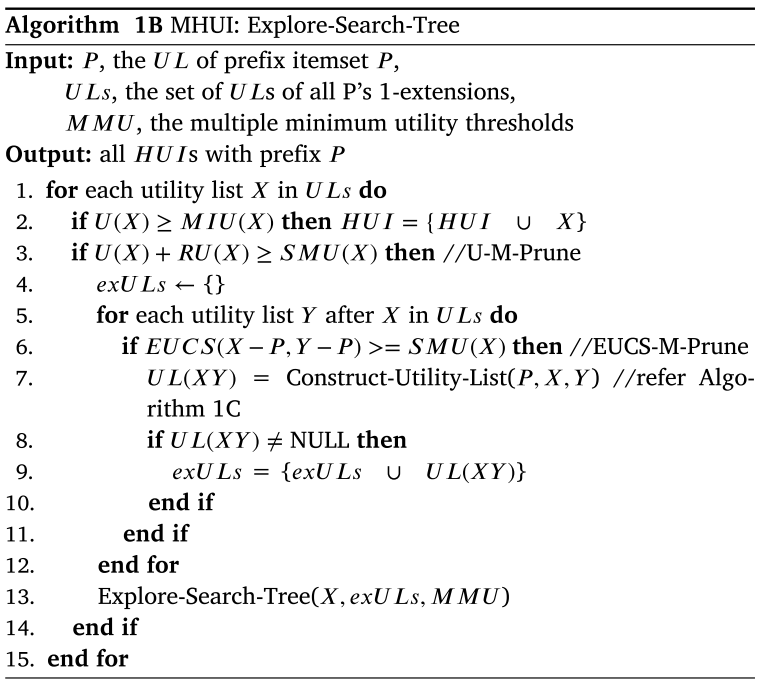
\includegraphics[width=0.9\textwidth]{image/algo/algo2.PNG}
\caption{\label{fig:algo2} MHUI Explore Search Tree}
\end{figure}

\paragraph{Dữ liệu đầu vào} Một itemset gọi là P, tập hợp có thứ tự các itemset ULs, ngưỡng giá trị hữu dụng tối thiểu cho từng món hàng.

\paragraph{Dữ liệu đầu ra} HUIs với tiền tố P \\

Hàm duyệt cây (hình \ref{fig:algo2}) sẽ kiểm tra cái nút tại đó xem nó có là HUI không (có $U(X) \geq MIU(X)$ ) đê gắn nút vào danh sách HUI trả về cuối cùng. Hàm duyệt cây theo Depth First Search, nghĩa là nó sẽ duyệt một nút sâu nhất có thể, sau đó mới chuyển qua nút tiếp theo. Một nút chỉ được duyệt khi nó thỏa U-M-Prune. 

Quá trình duyệt cây sẽ lập qua mỗi X trong tập ULs. Nếu X thóa U-M-Prune, rồi vòng lập con lập qua mỗi Y theo sau X trong ULs (ULs đã xếp theo thứ tự TWU), và thực hiện 2 việc sau 

\begin{itemize}
  \item kiểm tra P, X, Y thỏa EUCS-M-Prune (dòng 6), bỏ qua vòng lập này nếu không thỏa   
  \item xây dựng danh sách UL (dòng 7). Sẽ gọi hàm \ref{fig:algo3} để tạo ra UL. 
  \item gộp vào dãy exULs (dòng 8) 
\end{itemize}
 
Sau mỗi vòng lập ngoài (vòng lập của X) thuật toán gọi đệ quy gọi đệ quy Explore-Search-Tree(X, exULs) để duyệt cây theo depth first search. 

\subsubsection{Xây dựng dãy hữu dụng: Construct-Utility-List }

\paragraph{Dữ liệu đầu vào} UL itemset P, itemset Px, và itemset Py 

\paragraph{Dữ liệu đầu ra} UL của itemset Pxy \\

\begin{figure}[ht]
\centering
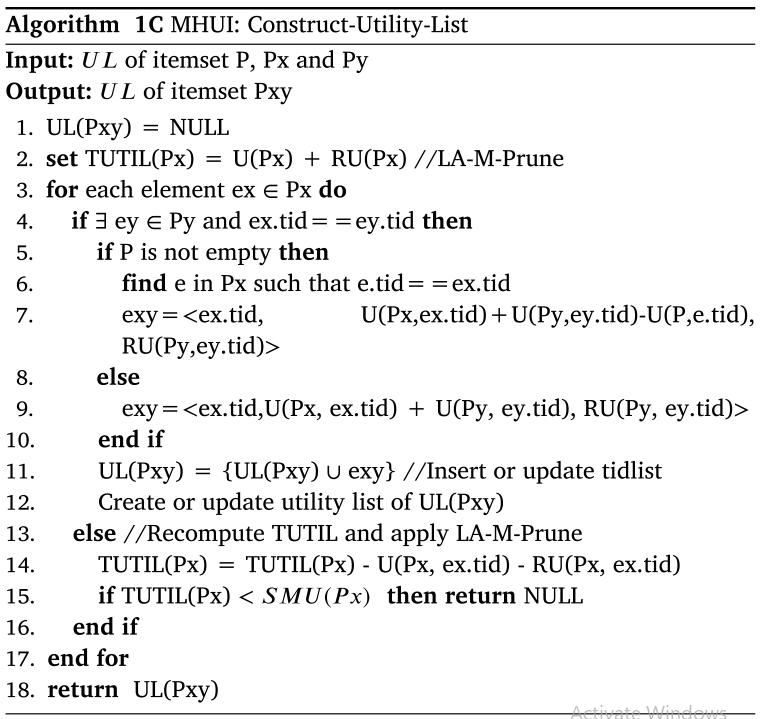
\includegraphics[width=0.9\textwidth]{image/algo/algo3.PNG}
\caption{\label{fig:algo3} MHUI Construct Utility List}
\end{figure}

Thuật toán tạo dãy Utility như hình \ref{fig:algo3} sẽ tạo ra UL mới từ 2 bằng cách ghép 2 UL Px và Py. Cả 2 UL Px và Py đều có chung tiền tố P. Thuật toán sẽ áp dụng LA-M-Prune và trả về NULL (rỗng) khi Px và Py không thỏa điều kiện. 

Kết quả trả về sẽ như một cột như hình \ref{fig:1itemset}, bao gồm itemset và mỗi dãy các bảng ghi có dạng <tid, U, RU>. 


\subsection{Các phương pháp cắt tỉa cây}

\paragraph{TWU-M-Prune} Nếu $TWU(X) < SMU(X)$ thì những itemset có chứa X (superset của X) không phải là HUI. TWU-M-Prune thực hiện ở dòng 6 trong hình \ref{fig:algo1}.

\paragraph{U-M-Prune} Nếu tổng giá trị tiện ích hậu tố của itemset X nhỏ hơn SMU(X) thì những itemset chứa X (superset của X) không phải HUI. Cụ thể $U(X) + RU(X) < SMU(X)$ thì những itemset chứa X không phải HUI. U-M-Prune thực hiện ở dòng 3 trong hình \ref{fig:algo2}.

\paragraph{EUCS-M-Prune} Nếu EUCS của 2-itemset X nhỏ hơn SMU(X) thì những itemset có chứa X (superset của X) không phải là HUI. 

\paragraph{LA-M-Prune} Phương pháp tỉa cây này sử dụng cả 2 itemset là X và Y, được dùng trong thuật toán xây dựng Utility List (hình \ref{fig:algo3}. Có thể hiểu như sau: 

\begin{itemize}
  \item Tính tổng = $U(X) + RU(X)$ (dòng 2)
  \item Nếu một giao dịch $T_j$ chứa itemset X mà không chứa itemset Y thì giảm tổng đi $U(X, T_j) + RU(X, T_j)$ (điều kiện if dòng 4, phép tính dòng 14) 
  \item Nếu tổng đó nhỏ hơn SMU(X) thì ta cắt bỏ X và kết luận những itemset có chứa X (superset của X) không phải là HUI
\end{itemize}


% % Commands to include a figure:
\begin{figure}[h]
\centering

\includegraphics[width=0.5\textwidth]{image/node.PNG}
\caption{\label{fig:node} Nút}
\end{figure}


% chuong 3
\section{Chèn đoạn code}


ví dụ code \ref{lst:vdcode} là code python 


\begin{lstlisting}[caption={Đoạn code}, label={lst:vdcode}, language=python]
s = "I am Pusheen the cat"
print(s)
\end{lstlisting}

ví dụ trích dẫn \cite{robinson2013graph}


\bibliographystyle{IEEEtran}
\bibliography{bib}

%%%%%%%%%%%%%%%%%%%%%%%%%%%%%%%%%%%%%%%%%%%%%%%%%%%%
% Comments can be added to the margins of the document using the \todo{Here's a comment in the margin!} todo command, as shown in the example on the right. You can also add inline comments too:

% \todo[inline, color=green!40]{This is an inline comment.}



% \subsection{Tables and Figures}

% Use the table and tabular commands for basic tables --- see Table~\ref{tab:widgets}, for example. You can upload a figure (JPEG, PNG or PDF) using the files menu. To include it in your document, use the includegraphics command as in the code for Figure~\ref{fig:frog} below.

% % % Commands to include a figure:
% % \begin{figure}
% % \centering
% % 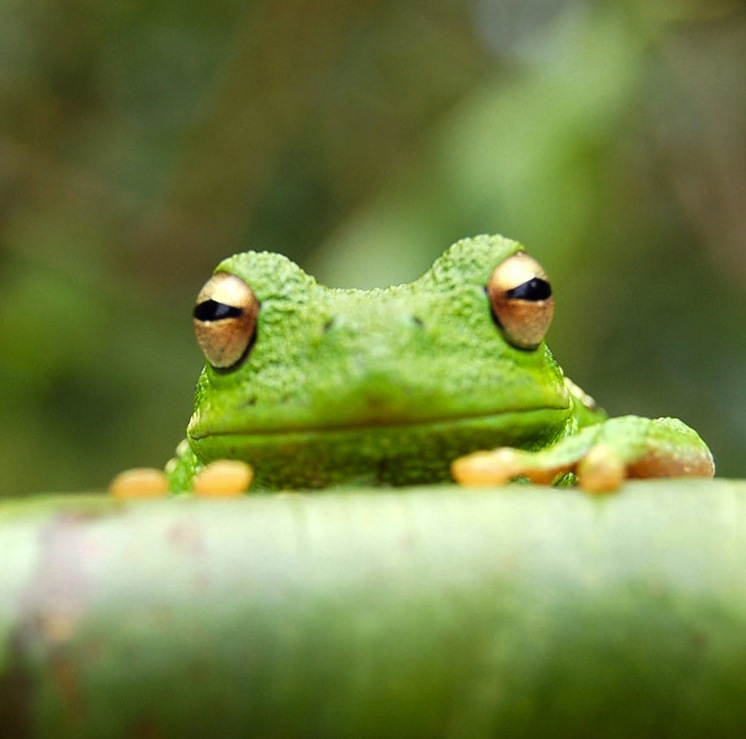
\includegraphics[width=0.5\textwidth]{frog.jpg}
% % \caption{\label{fig:frog}This is a figure caption.}
% % \end{figure}

% % \begin{table}
% % \centering
% % \begin{tabular}{l|r}
% % Item & Quantity \\\hline
% % Widgets & 42 \\
% % Gadgets & 13
% % \end{tabular}
% % \caption{\label{tab:widgets}An example table.}
% % \end{table}

% \subsection{Mathematics}

% \LaTeX{} is great at typesetting mathematics. Let $X_1, X_2, \ldots, X_n$ be a sequence of independent and identically distributed random variables with $\text{E}[X_i] = \mu$ and $\text{Var}[X_i] = \sigma^2 < \infty$, and let
% $$S_n = \frac{X_1 + X_2 + \cdots + X_n}{n}
%       = \frac{1}{n}\sum_{i}^{n} X_i$$
% denote their mean. Then as $n$ approaches infinity, the random variables $\sqrt{n}(S_n - \mu)$ converge in distribution to a normal $\mathcal{N}(0, \sigma^2)$.

% \subsection{Lists}

% You can make lists with automatic numbering \dots

% \begin{enumerate}
% \item Like this,
% \item and like this.
% \end{enumerate}
% \dots or bullet points \dots
% \begin{itemize}
% \item Like this,
% \item and like this.
% \end{itemize}

% We hope you find write\LaTeX\ useful, and please let us know if you have any feedback using the help menu above.

\end{document} to your LaTeX file where you want your
% title page.
%t
%%%%%%%%%%%%%%%%%%%%%%%%%%%%%%%%%%%%%%%%%
\title{Template báo cáo KHTN}
%----------------------------------------------------------------------------------------
%	PACKAGES AND OTHER DOCUMENT CONFIGURATIONS
%----------------------------------------------------------------------------------------

\documentclass[12pt]{article}
\usepackage[T5]{fontenc}
\usepackage[utf8]{inputenc}
\usepackage[vietnamese,english]{babel}
\usepackage{amsmath}
\usepackage{graphicx}
\usepackage[colorinlistoftodos]{todonotes}
\usepackage{listings}
\usepackage{hyperref}
\hypersetup{
    colorlinks=true,
    linkcolor=blue,
    filecolor=magenta,      
    urlcolor=cyan,
}

% change name 
\renewcommand{\lstlistingname}{Mã }% Listing -> Algorithm
\addto\captionsenglish{\renewcommand{\figurename}{Hình}} % figure -> Hình 

\usepackage{indentfirst} % thục dòng cái dòng đầu tiên 

\begin{document}

\begin{titlepage}

\newcommand{\HRule}{\rule{\linewidth}{0.5mm}} % Defines a new command for the horizontal lines, change thickness here

\center % Center everything on the page
 
%----------------------------------------------------------------------------------------
%	HEADING SECTIONS
%----------------------------------------------------------------------------------------

\textsc{\LARGE Đại học Khoa học tự nhiên}\\[1.5cm] % Name of your university/college
\textsc{\Large Ngành hệ thống thông tin}\\[0.5cm] % Major heading such as course name
\textsc{\large Môn học: Khám phá tri thức và khai thác dữ liệu }\\[0.5cm] % Minor heading such as course title

%----------------------------------------------------------------------------------------
%	TITLE SECTION
%----------------------------------------------------------------------------------------

\HRule \\[0.4cm]
{ \LARGE \bfseries Báo cáo cuối kỳ}\\[0.4cm]
{ \huge \bfseries Tìm hiểu bài báo}\\[0.2cm] % Title of your document
{ \huge \bfseries Efficient mining of high utility itemsets with multiple minimum utility thresholds}\\[0.4cm] % Title of your document
\HRule \\[1.5cm]
 
%----------------------------------------------------------------------------------------
%	AUTHOR SECTION
%----------------------------------------------------------------------------------------

\begin{minipage}{0.4\textwidth}
\begin{flushleft} \large
\emph{Học viên:}\\
Thái Thiện  -- 17C12031 % Your name
\end{flushleft}
\end{minipage}
~
\begin{minipage}{0.4\textwidth}
\begin{flushright} \large
\emph{Giảng viên:} \\
PGS.TS. LÊ HOÀI BẮC % Supervisor's Name
\end{flushright}
\end{minipage}\\[2cm]

% If you don't want a supervisor, uncomment the two lines below and remove the section above
%\Large \emph{Author:}\\
%John \textsc{Smith}\\[3cm] % Your name

%----------------------------------------------------------------------------------------
%	DATE SECTION
%----------------------------------------------------------------------------------------

% I don't want day because it is English
% {\large \today}\\[2cm] % Date, change the \today to a set date if you want to be precise

%----------------------------------------------------------------------------------------
%	LOGO SECTION
%----------------------------------------------------------------------------------------


\includegraphics{logo/rsz_3logo-khtn.png}\\[1cm] % Include a department/university logo - this will require the graphicx package
 
%----------------------------------------------------------------------------------------

\vfill % Fill the rest of the page with whitespace

\end{titlepage}


\section{Giới thiệu}
Báo cáo này sẽ trình bày về bài báo "Efficient mining of high utility itemsets with multiple minimum utility thresholds" \cite{krishnamoorthy2018efficient} của tác giả Srikumar Krishnamoorthy, thuộc đơn vị Học viện Quản lý Ahmedabad, Ấn Độ. Bài báo đăng trong tập chí Engineering Applications of Artificial Intelligence, năm 2018. 

Bài báo cung cấp một giải pháp cho bài toán khai tập hàng có hữu dụng cao (high utility itemset mining). Giải quyết bài toán này cho phép người ra quyết định khả năng linh hoạc khi sử dụng những giá trị hữu dụng của món hàng như lợi nhuận để khai thác những dấu hiệu từ cơ sở dữ liệu mà thông qua đó có thể đưa ra quyết định.  

Bài báo giới thiệu phương pháp tạo ra các tập hàng hữu dụng cao chỉ qua một bước mà không cần thông qua bước tạo các ứng cử viên tốn kém. Ngoài ra bài báo đề xuất một khái niệm gọi là tiền tố hữu dụng tối thiểu và phương pháp tỉa cây hiệu quả cho việc khai thác tập hàng có tính hữu dụng cao. 

Khai thác tập phổ biến hoặc có tính hữu dụng cao được áp dụng trong nhiều lĩnh vực như bán lẽ, nhà kho, thương mại điện tử, ngân hàng, bảo hiểm, chăm sóc sức khỏe. Tập phổ biến hoặc tập có tính hữu dụng cao giúp quản lý phân tích cách mà khách hàng mua sản phẩm hoặc nhu cầu, từ đó đề ra phương pháp vận hành kho bãi hiệu quả \cite{chen2005aggregation, chen2005association}.

\subsection{Đóng góp của bài báo}

Bài báo có các đóng góp chính sau

\begin{enumerate}
  \item Bài báo giới thiệu thuật toán mới, gọi là MHUI, giúp khai thác hiệu quả các tập hữu dụng cao (High utility itemset - HUI) với nhiều (theo từng món hàng) hạn mức hữu dụng tối thiểu. Bài toán sử dụng cơ sở dữ liệu hàng dọc để lưu trữ thông tin các tập hàng và khai thác HUI
  \item Bài báo giới thiệu khải niệm Hậu tố hữu dụng tối thiểu (Suffix Minimum Utility - SMU) để khai thác HUI hiệu quả. SMU được dùng thay thế cho phương pháp cắt tỉa vì các phương pháp cắt tỉa thông thường không còn phù hợp cho cách khai thác HUI được đề xuất này.
  \item Tác giả làm thí nghiệm so sánh MHUI với các phương pháp tối tân hiện nay trên 8 cơ sở dữ liệu thưa và dày để chứng tỏ MHUI có ích. Phương pháp MHUI nhanh hơn HUI-MMU-TE \cite{lin2016efficient} và HIMU-EUCP \cite{gan2016more} hàng trăm lần.  
\end{enumerate}

\subsection{Công trình liên quan}

\subsubsection{Tìm tập phổ biến: một và nhiều ngưỡng support}

Khai thác luật kết hợp (Association Rule Mining - ARM) là một bài toán được nghiên cứu rộng rãi trong lĩnh vực khai thác dữ liệu. Khai thác luật kết hợp gồm 2 bước. Bước đầu là khai thác các món hàng thường xuất hiện cùng nhau trong các giao dịch. Bước sau, khai thác luật từ các tập hàng phổ biến đã tạo ra. Một số thuật toán nổi tiến bao gồm Apriori\cite{agrawal1994fast}, FP-Growth\cite{han2000mining}, Eclat\cite{zaki2000scalable}. 

Thuật toán tìm tập hàng phổ biết thường chỉ có một hạn mức support nên thường bị vấn đề hàng hiếm \cite{liu1999mining}. Vì vậy, đã có một vài nghiên cứu về cách dùng nhiều hạn mức support. Một số thuật toán như MSApriori \cite{liu1999mining}, CFP-Growth \cite{hu2006mining}, CFP-Growth ++ \cite{kiran2011novel}, FP-ME \cite{gan2017mining}. Nhưng các phương pháp đó có những hạn chế như không thể áp dụng cho bài toán khai thác HUI có những đại lượng dùng tổng quát là giá trị hữu dụng như lợi nhuận, số lượng mua \cite{lin2016efficient}. 

\subsubsection{Khai thác tập hữu dũng cao : Một ngưỡng hữu dụng}

Khai thác tập hữu dụng (HUI mining) là một trong những chủ đề được nghiên cứu tích cực nhất trong mười năm nay. Vấn đề được nêu lên lần đầu bởi Liu và cộng sự (2005) để giải quyết hạn chế trong phương pháp khai thác luật kết hợp. Thuật toán hai bước \cite{liu2005two} đề xuất cách tạo ứng viên theo từng mức và cách kiểm chứng. Bước đầu, thuật toán khai thác tất cả nhóm hàng có giá trị hữu dụng theo trọng số giao dịch cao. Bước sau, giá trị hữu dụng của từng nhóm hàng được tính và nhóm không phải HUI bị lược bỏ. Các giải pháp tương tự như UMining and UMining\_H \cite{yao2006mining}, FUM and DCG+ \cite{li2008isolated}, GPA \cite{lan2012efficient}.

Thuật toán khai thác theo từng bật không mở rộng tốt với dữ liệu lớn hay dày. Nên một vài phương pháp tiếp cận dạng cây được nghiên cứu như IHUP \cite{ahmed2009efficient}, HUC-Prune \cite{ahmed2011huc}, UP-Growth \cite{tseng2010up}, UP-Growth+ \cite{tseng2013efficient}.

Các công trình gần đây sử dụng cấu trúc cơ sở dữ liệu dọc để khai thác HUI hiệu quả. Một cấu trúc dữ liệu dạng dãy hữu dụng để chứa thông tin về nhóm hàng. Một số công trình về dãy hữu dụng như HUI-Miner \cite{liu2012mining}, FHM \cite{fournier2014fhm}, HUP-Miner \cite{krishnamoorthy2015pruning}. Cách dùng dãy hữu dụng được chứng mình là tốt nhất vì nó không tạo ra ứng viên và sử dụng chiến thuật cắt tỉa hiệu quả \cite{fournier2014fhm} \cite{liu2012mining}. d2HUP \cite{liu2012mining} sử dụng cấu trúc dữ liệu hyperlink tên là CAUL để khai thac HUI hiệu quả.

Thuật toán EFIM \cite{zida2017efim} dùng cơ sở dữ liệu ngang để lưu thông tin về nhóm hàng. Thuật toán gộp các giao dịch trùng lấp trong cơ sở dữ liệu dày đặc. 

\section{Các định nghĩa về ký hiệu và bài toán}

\subsection{Định nghĩa}
% from def 1 -> 17

Cho tập $ I = \{i_1, i_2, ..., i_m\}$ là tập các món hàng (item) khác nhau. Một giao dịch (transaction) $T_j = \{x_l | 1, 2, ...N_j, x_l \in I \} $ với $N_j$ là số hàng trong giao dịch  $T_j$. Một cơ sở dữ liệu (database) $D$ có chứa các giao dịch, $D = \{T_1, T_2, ..., T_m\}$, với $m$ số các giao dịch trong cơ sở dữ liệu. Một tập hợp chưa các món hàng $X =\{ x_1, x_2, ... x_k \} \subset I, x_i \in I $ gọi là k-itemset. 

Hình \ref{fig:table2} là một cơ sở dữ liệu D chứa thông tin các giao dịchụ. Hình \ref{fig:table3} là lợi nhuận mỗi đơn vị của mỗi món hàng, và giá trị sử dụng tối thiểu được cho trước.



\begin{figure}[h]
\centering
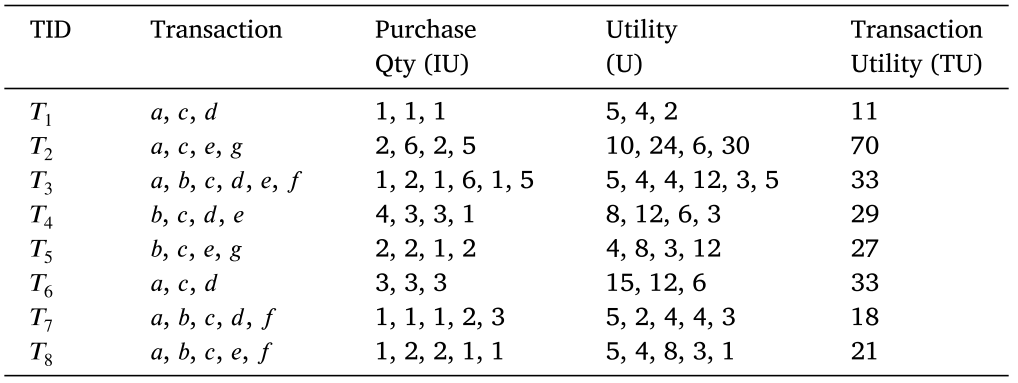
\includegraphics[width=0.9\textwidth]{image/table/table2.PNG}
\caption{\label{fig:table2} Cơ sở dữ liệu}
\end{figure}

\begin{figure}[h]
\centering
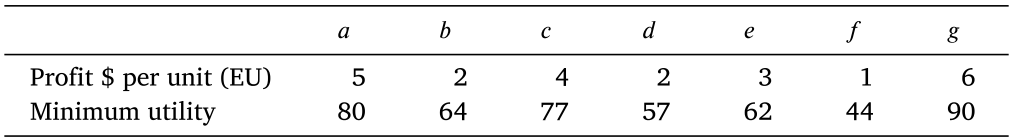
\includegraphics[width=0.9\textwidth]{image/table/table3.PNG}
\caption{\label{fig:table3} Lợi nhuận và giá trị sử dụng tối thiểu}
\end{figure}

\paragraph{Định nghĩa 1}: $ MU(x_i) $ là giá trị tiện ít tối thiểu (minimum utility threshold) của món hàng $x_i$. Thực tế, giá trị tiện ích tối thiểu của món hàng thể hiện hạn mức quan trọng của người dùng đối với món hàng đó. Trong quá trình khai thác, ta tính giá trị tiện ích của mỗi món hàng. Nếu giá trị tiện ích dưới giá trị tiện ích tối thiểu, ta không xét món hàng đó nữa. 

\paragraph{Định nghĩa 2} $MIU(X)$ là giá trị tiện ích tối thiểu của k-itemset, là $MU(x)$ với $x$ là món hàng có giá trị tiện ích tối thiểu nhỏ nhất. $MIU(X) = min \{MU(x_j|x_j \in X\}$ . Ví dụ: $MIU(a) = 80$, $MIU(af) = min\{MU(a), MU(f)\} = 44$


\paragraph{Định nghĩa 3} Chỉ số support của itemset X trong cơ sở dữ liệu D kí hiệu là $Sup(X)$. Support của itemset là tỉ lệ của tần số xuất hiện của itemsetX và tổng số giao dịch n. Ví dụ: $Sup(ac) = 6/8$

\paragraph{Định nghĩa 4} Mỗi món hàng $x_i \in I$ đều có giá trị tiện ích ngoài (external utility value), ký hiệu là $EU(x_i)$. Ví dụ: trong hình \ref{fig:table3} $EU(b) = 2$

\paragraph{Định nghĩa 5} Mỗi món hàng $x_i \in T_j$ có giá trị tiện ích bên trong (internal utility value), kí hiệu là $IU(x_i, T_j)$. Ví dụ: trong hình \ref{fig:table2}, $UI(b, T_3) = 2$

\paragraph{Định nghĩa 6} Giá trị tiện ích của món hàng $x_i \in T_j$ kí hiệu $U(x_i, T_j)$ là tích của giá trị tiện ích ngoài và giá trị tiện ích bên trong. 

$$ U(x_i, T_j) = EU(x_i) \times IU(x_i, T_j) $$ .

Ví dụ: $U(b, T_3) = EU(b) \times IU(b, T_3) = 2 \times 2 = 4$

Giá trị tiện ích thể hiện mức độ quan trọng của món hàng về số lượng được mua (giá trị tiện ích trong) và lợi nhuận mỗi đơn vị (giá trị tiện ích ngoài)

\paragraph{Định nghĩa 7} Giá trị tiện ích của itemset X trong giao dịch $T_j$ là tổng giá trị tiện ích của mỗi món hàng trong itemset đó. 
$$U(X, T_j) = \sum_{x_i \in X} U(x_i, T_j)$$
Ví dụ: trong hình \ref{fig:table2}, $U(ac, T_1) = 5 + 4 = 9$

\paragraph{Định nghĩa 8} $U(X)$ giá trị tiện ích của itemset X trong cơ sở dữ liệu D, bằng tổng giá trị tiện ích của itemset X trong mỗi giao dịch $T_j$

$$ U(X) = \sum_{x_i \subseteq T_j \in D} U(X, T_j) $$

Ví dụ: $U(ac) = U(ac, T_1) + U(ac, T_2) + U(ac, T_3) + U(ac, T_6) + U(ac, T_7) + U(ac, T_8) = 9 + 34 + 9 + 28 + 9 + 13 = 101 $

\paragraph{Định nghĩa 9} Tiện ích của giao dịch $TU(T_j)$ là tổng tiện ích của mỗi món hàng trong giao dịch j.

$$ TU(T_j) = \sum_{X \subseteq T_j and x_i \in X} U(x_i, T_j) $$

Ví dụ: $TU(T_5) = U(b, T_5) + U(c, T_5) + U(e, T_5) + U(g, T_5) = 27$

\paragraph{Định nghĩa 10}  $TWU(X)$ là trọng số giao dịch tiện ích (transaction weighted utility) của itemset X , bằng tổng tiện ích của các giao dịch có chứa itemset X.

$$ TWU(X) = \sum_{X \subseteq T_j \in D} TU(T_j) $$

Giá trị $TWU$ của từng món hàng ghi trong hình \ref{fig:table4}.



\begin{figure}[h]
\centering
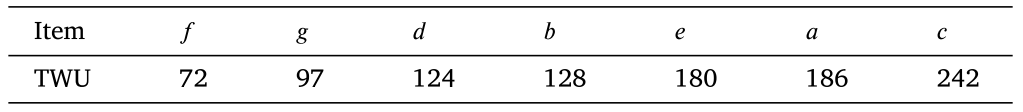
\includegraphics[width=0.9\textwidth]{image/table/table4.PNG}
\caption{\label{fig:table4} Trọng số giao dịch tiện ích  }
\end{figure}

\paragraph{Định nghĩa 11} $T_j/X$ là tập hợp các món hàng sau $X$ trong $T_j$. Ví dụ: trong hình \ref{fig:table2}, $T_i/ac = d, T_7/ac = df$.

\paragraph{Định nghĩa 12} $RU(X, T_j)$  là tiện ích còn lại (remaining utility) của itemset X trong giao dịch $T_j(X \subseteq T_j)$.

$$ RU(X, T_j) = \sum_{x_i \in (T_j/X)} U(x_i, T_j) $$

Ví dụ, trong hình \ref{fig:table2}, $RU(ac, T_1) = 2, RU(ac, T_7) = 4 + 3 = 7 $  

\paragraph{Định nghĩa 13} $RU(X)$ là tiện ích còn lại của itemset X trong cơ sở dữ liệu D, tính bằng tổng các tiện ích còn lại của X ở mỗi giao dịch $T_j$

$$ RU(X) = \sum_{X \subseteq T_j \in D} RU(x, T_j) $$

Ví dụ, trong hình \ref{fig:table2}, $RU(ac) = 2 + 36 + 20 + 6 + 7 + 4 = 75$

\paragraph{Định nghĩa 14} (Về thứ tự các món hàng). Các món hàng trong cơ sở dữ liệu các giao dịch được xử lý theo thứ tự $\succ$ xếp theo giá trị TWU tăng dần. Trong ví dụ của bài báo thứ tự là $ f \succ g \succ d \succ b \succ e \succ a \succ c $. Hình \ref{fig:table5} là cơ sở dữ liệu với mỗi giao dịch đã được sắp xếp các món hàng theo thứ tự TWU. 

\begin{figure}[h]
\centering
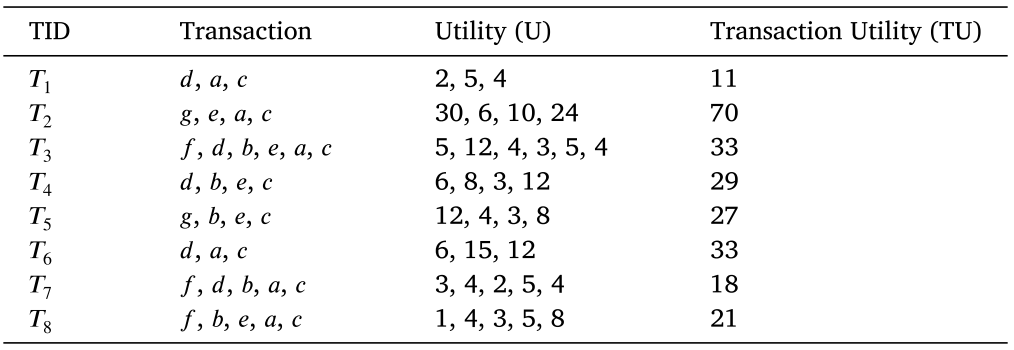
\includegraphics[width=0.9\textwidth]{image/table/table5.PNG}
\caption{\label{fig:table5} Cơ sở dữ liệu sau khi sắp xếp theo TWU  }
\end{figure}

\paragraph{Định nghĩa 15} (Về phần mở rộng của itemset). $Ext(X)$ là phần mở rộng của itemset X, là tất cả các món hàng sau X trong tập hợp các món hàng được xếp theo thứ tự. Ví dụ: $Ext(b) = \{ e, a, c \}$ và $Ext(fd) = \{b, e, a, c \}$.

\paragraph{Định nghĩa 16} $SMU(X)$ là hậu tố tiện ích tối thiểu (suffix minimum utility) của X. 

$$ SMU(U) = min(MIU(X), MIU(Ext(X))) $$

Ví dụ, $SMU(ea) = min(MIU(ea), MIU(Ext(ea))) = min (MIU(ea), MIU(c)) = min(min(62, 80), 77) = 62$

\paragraph{Định nghĩa 17} EUCS, cấu trúc đồng xảy ra tiện ích ước tính (Estimated Utility Co-occurrence Structure) \cite{fournier2014fhm} là một ma trận tam giác như hình \ref{fig:eucs}. Ma trận này để chứa giá trị TWU của một cặp itemset. 

\begin{figure}[h]
\centering
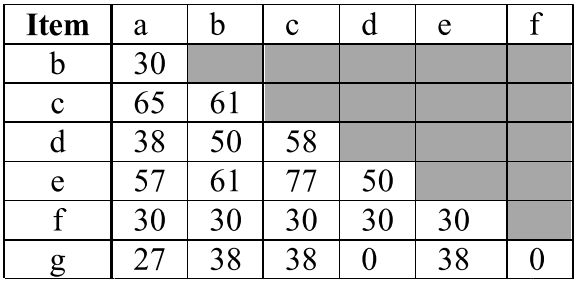
\includegraphics[width=0.7\textwidth]{image/fig/trianglematrix.PNG}
\caption{\label{fig:eucs} Ma trận tam giác  }
\end{figure} 

\subsection{Định nghĩa bài toán}

\paragraph{Dữ liệu đầu vào} Cơ sở dữ liệu D chứa các giao dịch, $D = \{T_1, T_2, ..., T_m\}$, giá trị hữu dụng trong và ngoài của mỗi món hàng, và ngưỡng giá trị hữu dụng tối thiểu. (như trong hình \ref{fig:table2} và hình \ref{fig:table3}).

\paragraph{Dữ liệu đầu ra} Tập HUI (high utility itemset) bao gồm các itemset X có giá trị hữu dụng cao hơn giá trị hữu dụng tối thiểu của itemset đó (như hình \ref{fig:table6}). HUI định nghĩa như sau

$$HUI = \{ X : U(X) | X \subseteq I, U(X) \geq MIU(X) \} $$

\begin{figure}[h]
\centering
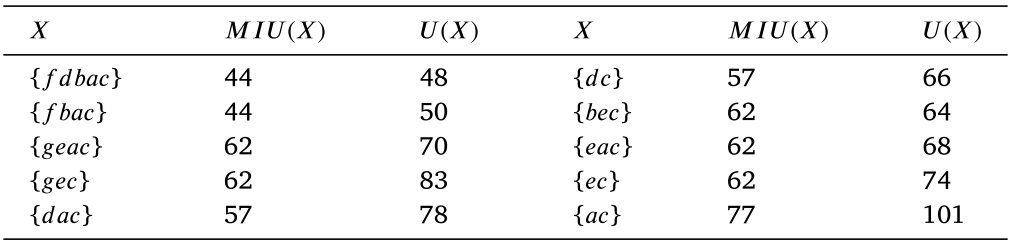
\includegraphics[width=0.9\textwidth]{image/table/table6.PNG}
\caption{\label{fig:table6} Tập HUI kết quả}
\end{figure}

\begin{figure}[h]
\centering
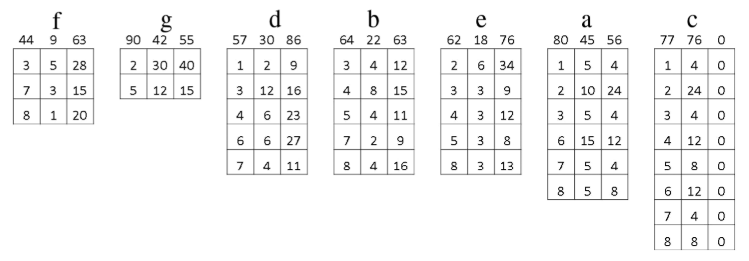
\includegraphics[width=0.95\textwidth]{image/algo/1itemset.PNG}
\caption{\label{fig:1itemset} Bảng 1-itemset}
\end{figure}

\section{Thuật toán MHUI}

\subsection{Mã giả các thuật toán}


\subsubsection{MHUI main}

\begin{figure}[ht]
\centering
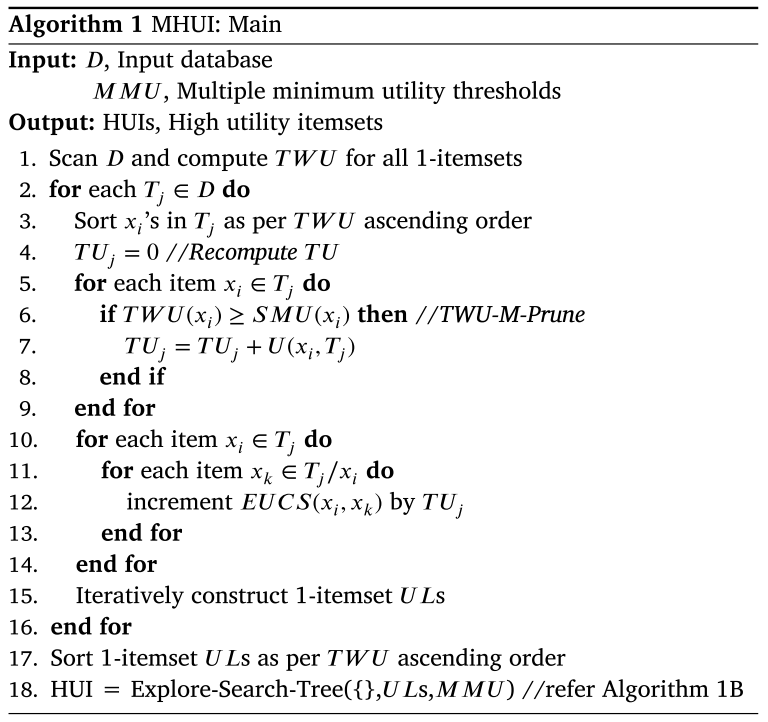
\includegraphics[width=0.9\textwidth]{image/algo/algo1.PNG}
\caption{\label{fig:algo1} MHUI main}
\end{figure}

\paragraph{Dữ liệu đầu vào} Cơ sở dữ liệu D, ngưỡng giá trị hữu dụng tối thiểu cho từng món hàng.  
\paragraph{Dữ liệu đầu ra} HUIs, tập các itemset có giá trị hữu dụng cao.\\



Hình \ref{fig:algo1} là hàm bắt đầu chương trình. Chương trình sẽ tính các TWU (tạo ra bảng như hình\ref{fig:table4}), dòng 1 trong thuật toán, đây là lần duyệt cơ sở dữ liệu đầu tiên. Sau đó, chương trình duyệt qua cơ sở dữ liệu lần 2, ở mỗi giao dịch $T_j$ chương trình sẽ làm những việc sau đây trong mỗi vòng lập qua 1 giao dịch.

\begin{itemize}
  \item Sắp xếp các món hàng trong giao dịch theo thứ tự TWU (dòng 3). 
  \item Tính lại TU cho mỗi giao dịch sau khi áp dụng phương pháp tỉa cây TWU-M-Prune. (dòng 6, 7)
  \item Tính EUCS dựa vào TU sau khi tỉa cây TWU-M-Prune (dòng 12)
  \item Từ từ xây dựng 1-itemset utility list (gọi tắt ULs) như hình \ref{fig:1itemset} (dòng 15) 
\end{itemize}

Sau khi kết thức vòng lập, sắp xếp ULs theo thứ tự TWU (dòng 17), gọi hàm Explore-Search-Tree (dòng 18). 

\subsubsection{Hàm duyệt cây: Explore-Search-Tree }

\begin{figure}[ht]
\centering
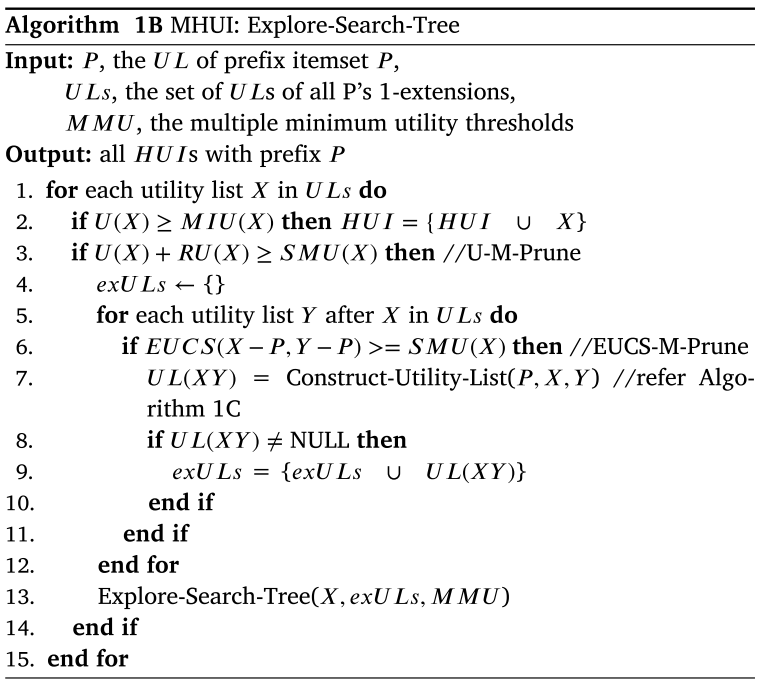
\includegraphics[width=0.9\textwidth]{image/algo/algo2.PNG}
\caption{\label{fig:algo2} MHUI Explore Search Tree}
\end{figure}

\paragraph{Dữ liệu đầu vào} Một itemset gọi là P, tập hợp có thứ tự các itemset ULs, ngưỡng giá trị hữu dụng tối thiểu cho từng món hàng.

\paragraph{Dữ liệu đầu ra} HUIs với tiền tố P \\

Hàm duyệt cây (hình \ref{fig:algo2}) sẽ kiểm tra cái nút tại đó xem nó có là HUI không (có $U(X) \geq MIU(X)$ ) đê gắn nút vào danh sách HUI trả về cuối cùng. Hàm duyệt cây theo Depth First Search, nghĩa là nó sẽ duyệt một nút sâu nhất có thể, sau đó mới chuyển qua nút tiếp theo. Một nút chỉ được duyệt khi nó thỏa U-M-Prune. 

Quá trình duyệt cây sẽ lập qua mỗi X trong tập ULs. Nếu X thóa U-M-Prune, rồi vòng lập con lập qua mỗi Y theo sau X trong ULs (ULs đã xếp theo thứ tự TWU), và thực hiện 2 việc sau 

\begin{itemize}
  \item kiểm tra P, X, Y thỏa EUCS-M-Prune (dòng 6), bỏ qua vòng lập này nếu không thỏa   
  \item xây dựng danh sách UL (dòng 7). Sẽ gọi hàm \ref{fig:algo3} để tạo ra UL. 
  \item gộp vào dãy exULs (dòng 8) 
\end{itemize}
 
Sau mỗi vòng lập ngoài (vòng lập của X) thuật toán gọi đệ quy gọi đệ quy Explore-Search-Tree(X, exULs) để duyệt cây theo depth first search. 

\subsubsection{Xây dựng dãy hữu dụng: Construct-Utility-List }

\paragraph{Dữ liệu đầu vào} UL itemset P, itemset Px, và itemset Py 

\paragraph{Dữ liệu đầu ra} UL của itemset Pxy \\

\begin{figure}[ht]
\centering
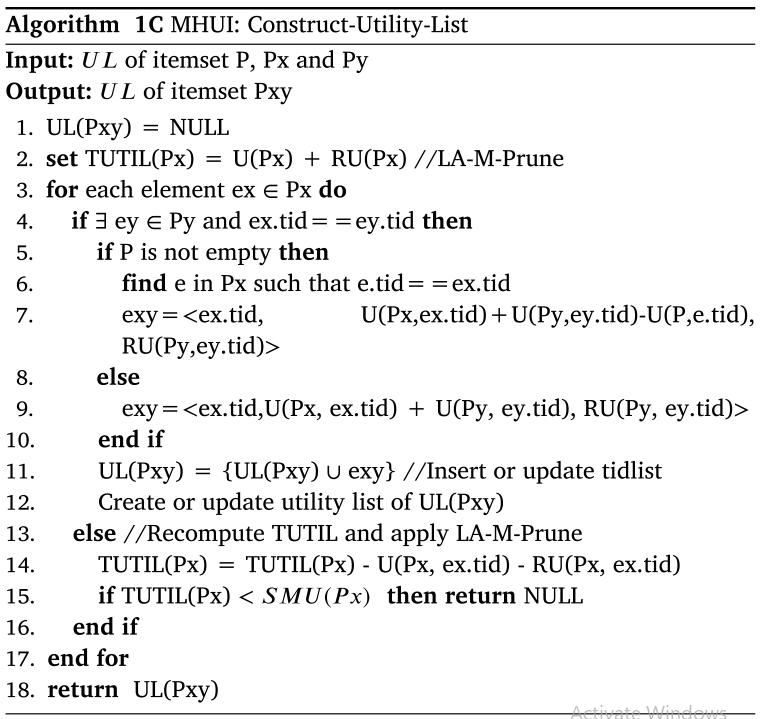
\includegraphics[width=0.9\textwidth]{image/algo/algo3.PNG}
\caption{\label{fig:algo3} MHUI Construct Utility List}
\end{figure}

Thuật toán tạo dãy Utility như hình \ref{fig:algo3} sẽ tạo ra UL mới từ 2 bằng cách ghép 2 UL Px và Py. Cả 2 UL Px và Py đều có chung tiền tố P. Thuật toán sẽ áp dụng LA-M-Prune và trả về NULL (rỗng) khi Px và Py không thỏa điều kiện. 

Kết quả trả về sẽ như một cột như hình \ref{fig:1itemset}, bao gồm itemset và mỗi dãy các bảng ghi có dạng <tid, U, RU>. 


\subsection{Các phương pháp cắt tỉa cây}


\paragraph{TWU-M-Prune} Nếu $TWU(X) < SMU(X)$ thì những itemset có chứa X (superset của X) không phải là HUI. TWU-M-Prune thực hiện ở dòng 6 trong hình \ref{fig:algo1}.

\paragraph{U-M-Prune} Nếu tổng giá trị hữu dụng hậu tố của itemset X nhỏ hơn SMU(X) thì những itemset chứa X (superset của X) không phải HUI. Cụ thể $U(X) + RU(X) < SMU(X)$ thì những itemset chứa X không phải HUI. U-M-Prune thực hiện ở dòng 3 trong hình \ref{fig:algo2}.

\paragraph{EUCS-M-Prune} Nếu EUCS của 2-itemset X nhỏ hơn SMU(X) thì những itemset có chứa X (superset của X) không phải là HUI. 

\paragraph{LA-M-Prune} Phương pháp tỉa cây này sử dụng cả 2 itemset là X và Y, được dùng trong thuật toán xây dựng Utility List (hình \ref{fig:algo3}. Có thể hiểu như sau: 

\begin{itemize}
  \item Tính tổng = $U(X) + RU(X)$ (dòng 2)
  \item Nếu một giao dịch $T_j$ chứa itemset X mà không chứa itemset Y thì giảm tổng đi $U(X, T_j) + RU(X, T_j)$ (điều kiện if dòng 4, phép tính dòng 14) 
  \item Nếu tổng đó nhỏ hơn SMU(X) thì ta cắt bỏ X và kết luận những itemset có chứa X (superset của X) không phải là HUI
\end{itemize}


% % % Commands to include a figure:
% \begin{figure}[h]
% \centering
% 
\includegraphics[width=0.5\textwidth]{image/node.PNG}
% \caption{\label{fig:node} Nút}
% \end{figure}


% % chuong 3
% \section{Chèn đoạn code}


% ví dụ code \ref{lst:vdcode} là code python 


% \begin{lstlisting}[caption={Đoạn code}, label={lst:vdcode}, language=python]
% s = "I am Pusheen the cat"
% print(s)
% \end{lstlisting}

% ví dụ trích dẫn \cite{robinson2013graph}


\bibliographystyle{IEEEtran}
\bibliography{bib}

%%%%%%%%%%%%%%%%%%%%%%%%%%%%%%%%%%%%%%%%%%%%%%%%%%%%
% Comments can be added to the margins of the document using the \todo{Here's a comment in the margin!} todo command, as shown in the example on the right. You can also add inline comments too:

% \todo[inline, color=green!40]{This is an inline comment.}



% \subsection{Tables and Figures}

% Use the table and tabular commands for basic tables --- see Table~\ref{tab:widgets}, for example. You can upload a figure (JPEG, PNG or PDF) using the files menu. To include it in your document, use the includegraphics command as in the code for Figure~\ref{fig:frog} below.

% % % Commands to include a figure:
% % \begin{figure}
% % \centering
% % 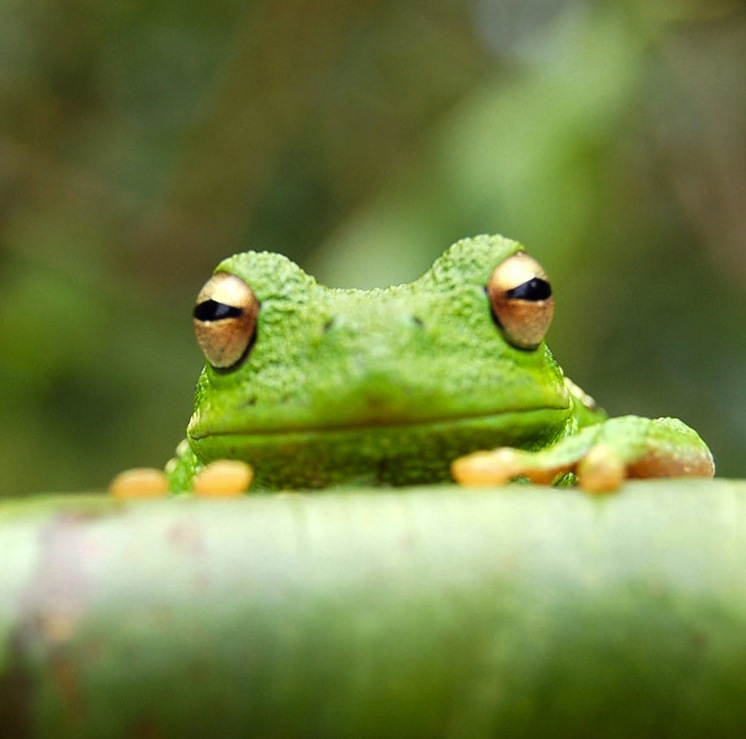
\includegraphics[width=0.5\textwidth]{frog.jpg}
% % \caption{\label{fig:frog}This is a figure caption.}
% % \end{figure}

% % \begin{table}
% % \centering
% % \begin{tabular}{l|r}
% % Item & Quantity \\\hline
% % Widgets & 42 \\
% % Gadgets & 13
% % \end{tabular}
% % \caption{\label{tab:widgets}An example table.}
% % \end{table}

% \subsection{Mathematics}

% \LaTeX{} is great at typesetting mathematics. Let $X_1, X_2, \ldots, X_n$ be a sequence of independent and identically distributed random variables with $\text{E}[X_i] = \mu$ and $\text{Var}[X_i] = \sigma^2 < \infty$, and let
% $$S_n = \frac{X_1 + X_2 + \cdots + X_n}{n}
%       = \frac{1}{n}\sum_{i}^{n} X_i$$
% denote their mean. Then as $n$ approaches infinity, the random variables $\sqrt{n}(S_n - \mu)$ converge in distribution to a normal $\mathcal{N}(0, \sigma^2)$.

% \subsection{Lists}

% You can make lists with automatic numbering \dots

% \begin{enumerate}
% \item Like this,
% \item and like this.
% \end{enumerate}
% \dots or bullet points \dots
% \begin{itemize}
% \item Like this,
% \item and like this.
% \end{itemize}

% We hope you find write\LaTeX\ useful, and please let us know if you have any feedback using the help menu above.

\end{document}